\chapter{Методи формалізації голосової інформації в системах диспетчерського контролю за рухом автотранспорту} \label{chapt3}

\section{Класифікація реакцій в системах диспетчерського контролю за рухом автотранспорту} \label{sect3_1}

Для виконання класифікації реакцій в системах диспетчерського контролю за рухом автотранспорту були зібрані статистичні дані (зауваження та коментарі) щодо процесу доставки різних вантажів автомобільним транспортом у провідних логістичних компаніях. Систематизувавши та обробивши зібрані оригінальні коментарі до статусу доставки, що використовуються в різних компаніях (табл. \ref{tbl:original_comments}) , виконано та запропоновано класифікацію для субʼєктів дистрибуції «склад – дорога – точка доставки» відповідно до моделі, що наведена на рис. \ref{img:voice_interaction_schema} та приведена нижче.

Для «складу» існують такі головні коментарі:
\begin{itemize}
	\item проблеми з вантажем:
	\begin{itemize}
		\item відсутня частина товару на складі;
		\item забруднена продукція (пил, бруд, стійкий сторонній запах);
		\item частина товару пошкоджена;
		\item немає накладної;
		\item неправильно розрахований тоннаж та/або обʼєм продукції (товар не вміщується в авто);
	\end{itemize}
	\item проблеми з машиною:
	\begin{itemize}
		\item поломка ТЗ;
		\item машина не заводиться;
	\end{itemize}
	\item проблеми з виїздом:
	\begin{itemize}
		\item запізнення прибуття на склад;
		\item затримка завантаження товару на складі за умови вчасної подачі автомобіля;
	\end{itemize}
	\item інші команди:
	\begin{itemize}
		\item набрати диспетчера;
		\item показати маршрутний лист;
		\item показати мапу маршруту;
		\item виїзд зі складу ->
	\end{itemize}
\end{itemize}

Для «дороги» існують такі головні коментарі:
\begin{itemize}
	\item неможливо досягти точку:
	\begin{itemize}
		\item заблокований вʼїзд/виїзд автомобіля доставки;
		\item немає підʼїзду до будинку (будів., дорожні роботи, припаркований транспорт і т.д.) обʼїхати неможливо;
		\item неправильна адреса, або недостатньо інформації для доставки замовлення;
		\item не знайшли адресу;
		\item не було місця для парковки;
		\item авто не пройшло по габаритам;
	\end{itemize}
	\item складнощі з досягненням точки:
	\begin{itemize}
		\item неправильне присвоєння сектору/координат;
		\item похибка при складанні маршруту (адреса точки доставки випадає з логіки загального маршруту);
		\item підʼїзд до будинку з іншої вулиці;
	\end{itemize}
	\item затримки у русі, відхилення від маршруту, можливо необхідний перерахунок маршруту:
	\begin{itemize}
		\item транспортний затор на маршруті;
		\item будів., дорожні роботи, перекриті дороги;
		\item помилка карти - маршрут прокладений по неіснуючій дорозі;
	\end{itemize}
	\item неможливо продовжувати маршрут:
	\begin{itemize}
		\item транспортний засіб попав у ДТП;
		\item поломка ТЗ на маршруті;
		\item складні погодні умови (автотранспорт фізично не може доїхати до місця доставки);
	\end{itemize}
	\item інші команди:
	\begin{itemize}
		\item набрати диспетчера;
		\item набрати клієнта;
		\item показати маршрутний лист;
		\item показати мапу маршруту;
		\item показати інформацію про точку;
		\item прибув у точку ->
	\end{itemize}
\end{itemize}

Для «точки доставки» існують такі головні коментарі:
\begin{itemize}
	\item відсутність клієнта:
	\begin{itemize}
		\item клієнт забув про доставку;
		\item особисті причини (клієнт не зміг бути вчасно);
		\item немає на місці, немає звʼязку (некоректний номер телефону для звʼязку, недозвон);
		\item невчасний (запізнення/достроковий) приїзд на точку доставку, клієнт не має змоги прийняти товар;
	\end{itemize}
	\item немає можливості виконати доставку:
	\begin{itemize}
		\item не працює ліфт, клієнт проживає вище Х поверху;
		\item закрито доступ до приміщення клієнта;
		\item у клієнта відсутні необхідні документи, матеріали чи товар для відвантаження;
	\end{itemize}
	\item відмова клієнта прийняти товар:
	\begin{itemize}
		\item відмова на місці;
		\item немає грошей;
		\item пошкоджений або відсутній товар:
		\begin{itemize}
			\item товар не завантажено;
			\item товар забруднений;
			\item товар недоукомплектован;
			\item товар не працює (внутрішня поломка);
			\item товар пошкоджено зовні;
		\end{itemize}
	\end{itemize}
	\item помилка в замовленні:
	\begin{itemize}
		\item не замовляли взагалі;
		\item замовляли на інший день;
		\item замовляли на іншу адресу;
		\item замовляли на інший час;
		\item замовляли інший товар;
	\end{itemize}
	\item часткове виконання замовлення:
	\begin{itemize}
		\item задвоєне замовлення, половина повертається;
		\item у документах зазначено товар, який клієнт не замовляв;
	\end{itemize}
	\item інші команди:
	\begin{itemize}
		\item набрати диспетчера;
		\item набрати клієнта;
		\item показати маршрутний лист;
		\item показати мапу маршруту;
		\item показати інформацію про точку;
		\item почав виконання наступної точки ->
		\item точка успішно виконана ->
	\end{itemize}
\end{itemize}

\section{Модель голосової взаємодії водія в системах диспетчерського контролю за рухом автотранспорту} \label{sect3_2}

\subsection{Побудова орієнтованого графу сценаріїв голосової взаємодії}

Як зазначалось в попередньому розділі, дерево сценаріїв може бути застосоване для голосової взаємодії субʼєктів дистрибуції «склад – дорога – точка доставки» відповідно до моделі, що наведена на рис. \ref{img:voice_interaction_schema}. Найпростіше дерево сценаріїв для моделі голосової взаємодії водія в системах диспетчерського контролю за рухом автотранспорту можна представити наступним чином (рис. \ref{img:01_simplest_positive_scenario}).

\begin{figure}
	\centering
	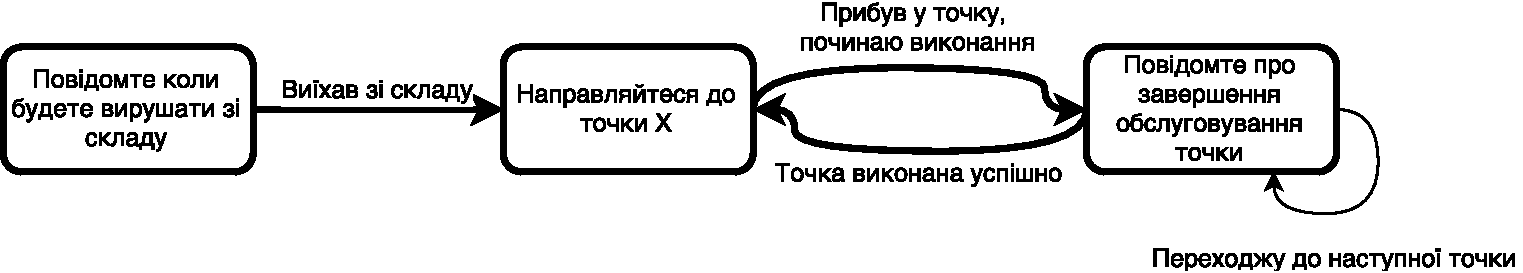
\includegraphics [width=1\linewidth] {01_simplest_positive_scenario}
	\caption{Найпростіше дерево сценаріїв}
	\label{img:01_simplest_positive_scenario}
\end{figure}

Таке ж найпростіше дерево сценаріїв для моделі голосової взаємодії водія в системах диспетчерського контролю за рухом автотранспорту тільки з вертикальним розподілом приведено на рис. \ref{img:02_simplest_positive_scenario_vertical}.

\begin{figure}
	\centering
	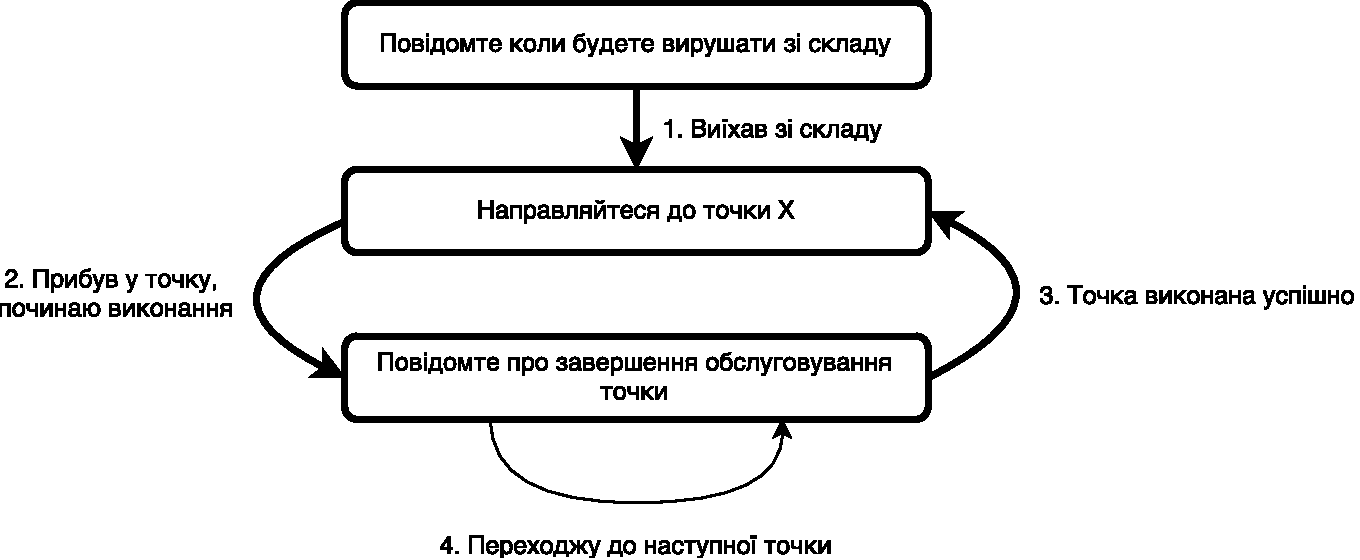
\includegraphics [width=1\linewidth] {02_simplest_positive_scenario_vertical}
	\caption{Вертикальний розподіл найпростішого дерева сценаріїв}
	\label{img:02_simplest_positive_scenario_vertical}
\end{figure}

Найпростіше дерево сценаріїв (рис. \ref{img:01_simplest_positive_scenario}, \ref{img:02_simplest_positive_scenario_vertical}) показує всі доступні варіанти (послідовність подій) у моделі голосової взаємодії водія в системах диспетчерського контролю за рухом автотранспорту. Кожна така послідовність або ланцюжок подій повинен представлятися окремим сценарієм.

Для випадку позитивного підтвердження обслуговування або виконання відповідної точки у моделі голосової взаємодії водія в системах диспетчерського контролю за рухом автотранспорту побудовано позитивне дерево сценаріїв (рис. \ref{img:03_positive_scenario_with_conformation}).

\begin{figure}
	\centering
	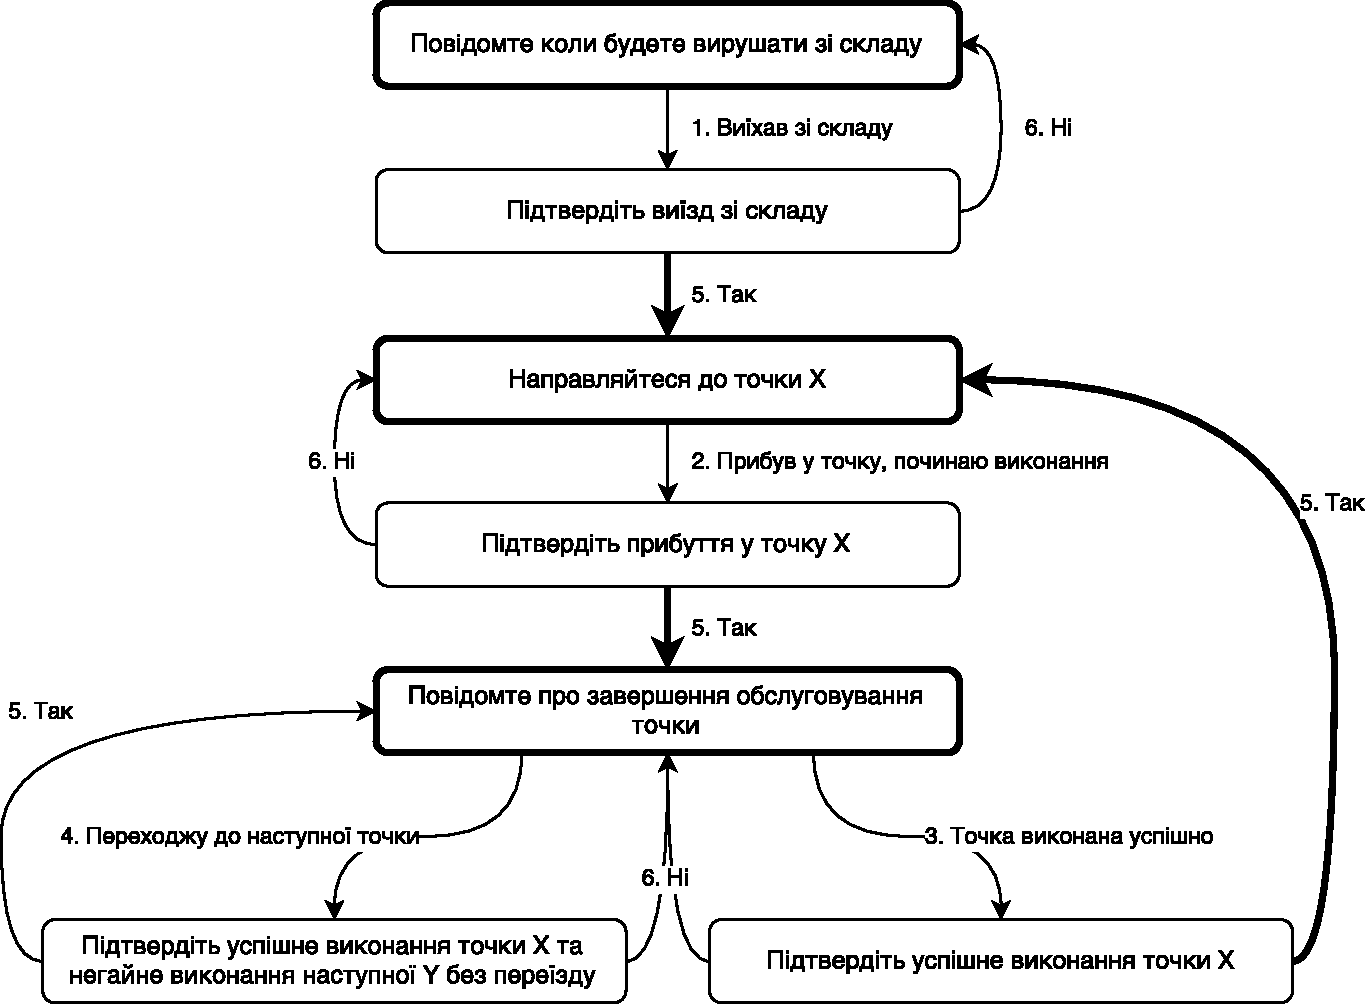
\includegraphics [width=1\linewidth] {03_positive_scenario_with_conformation}
	\caption{Позитивне дерево сценаріїв з підтвердженням}
	\label{img:03_positive_scenario_with_conformation}
\end{figure}

Наведене позитивне дерево сценаріїв з підтвердженням обслуговування або виконання відповідної точки (рис. \ref{img:03_positive_scenario_with_conformation}) є більш складним у порівнянні з найпростішим деревом сценаріїв (рис. \ref{img:01_simplest_positive_scenario}, \ref{img:02_simplest_positive_scenario_vertical}). Воно є достатнім в якомусь ідеальному світі, де все відбувається за планом. Це ключова відмінність цього дерева від попереднього, де врахована можливість помилки розпізнавання команди (чи помилкової команди від водія) Як бачимо, для даного випадку, обслуговування або виконання відповідної точки відбувається без проблем, на відміну від дерева сценаріїв з негативними інцидентами, перший варіант якого наведено на рис. \ref{img:04_first_negative_scenario_with_conformation}. 

На рис. \ref{img:04_first_negative_scenario_with_conformation} зʼявляється додатковий блок, повʼязаний з підтвердженням того, що точку Х не вдалося виконати, тобто дерево сценаріїв включає можливі негативні інциденти в моделі голосової взаємодії водія в системах диспетчерського контролю за рухом автотранспорту.

\begin{figure}
	\centering
	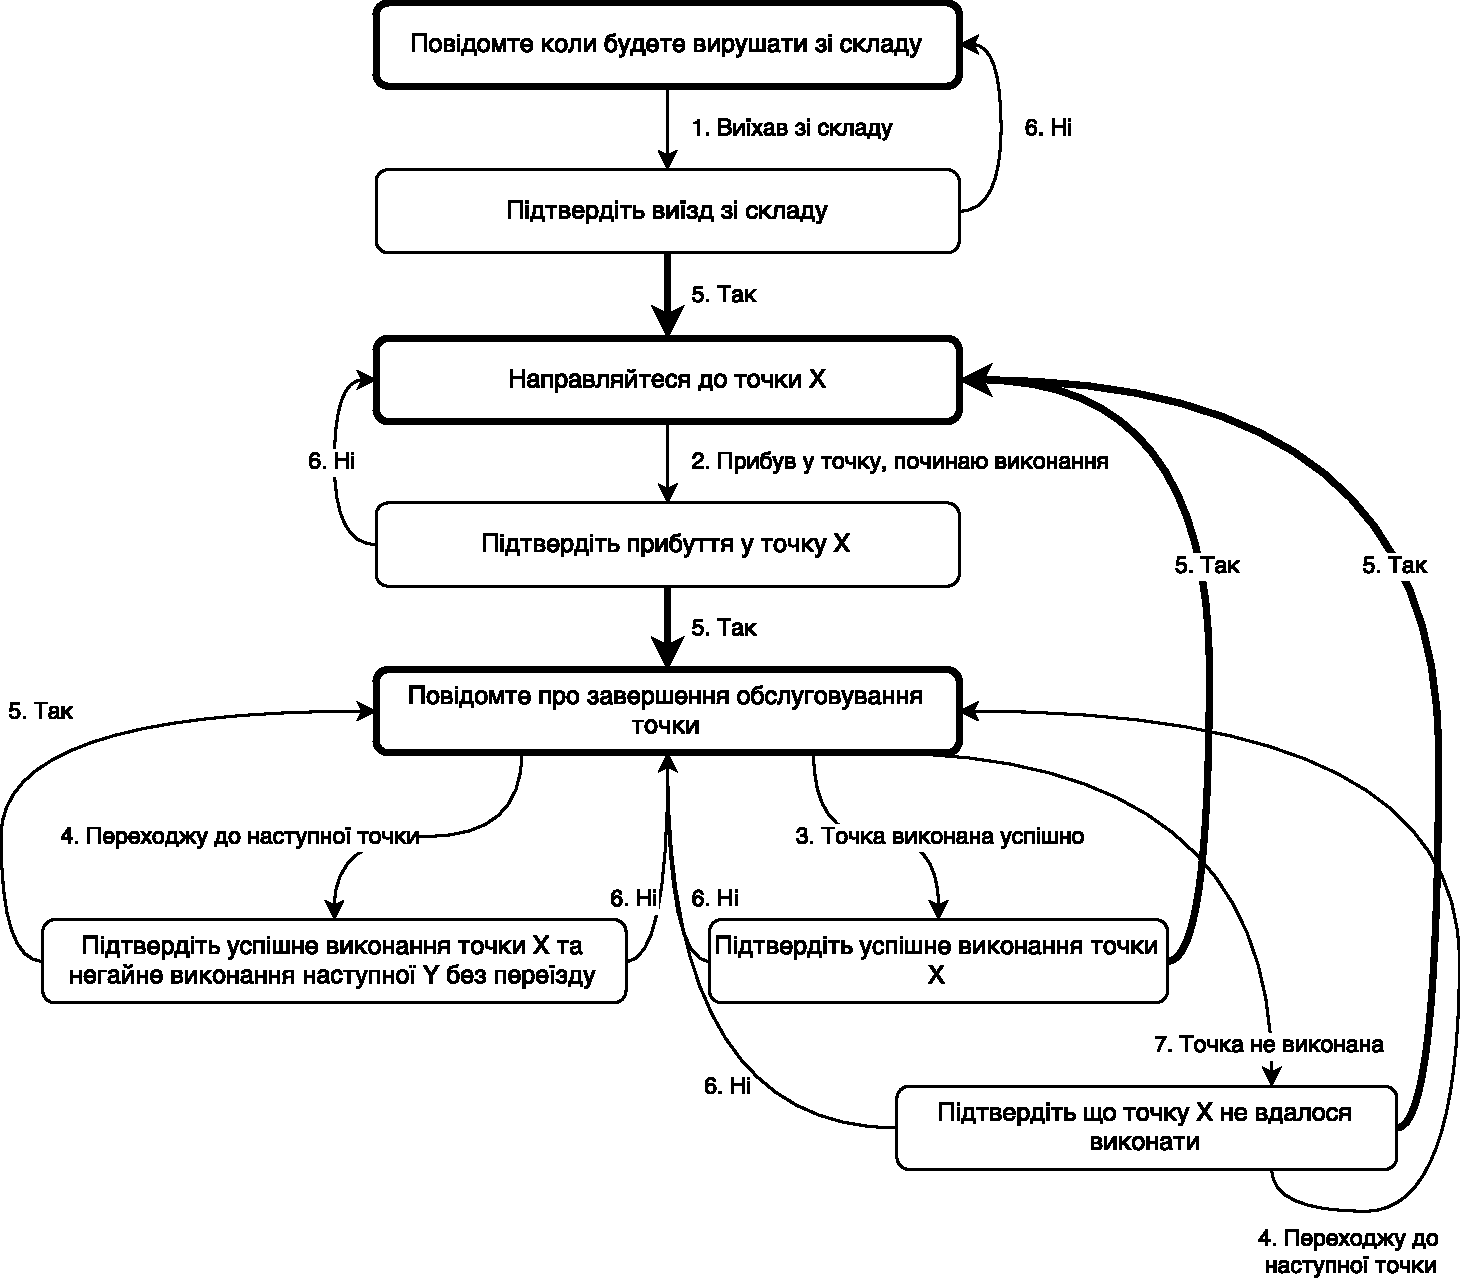
\includegraphics [width=1\linewidth] {04_first_negative_scenario_with_conformation}
	\caption{Перший варіант дерева сценаріїв з негативними інцидентами}
	\label{img:04_first_negative_scenario_with_conformation}
\end{figure}

Спрощений варіант дерева сценаріїв у моделі голосової взаємодії водія в системах диспетчерського контролю за рухом автотранспорту з негативними інцидентами наведено на рис. \ref{img:05_simple_negative_scenario_with_conformation}. У цьому варіанті блок з підтвердженням успішного виконання точки Х з негайним виконанням наступної точки Y без переїзду трансформується у блок, повʼязаний з підтвердженням того, що точку Х не вдалося виконати і стає, по-суті, спрощеним варіантом дерева сценаріїв з негативними інцидентами, що приведено на рис. \ref{img:04_first_negative_scenario_with_conformation}.

\begin{figure}
	\centering
	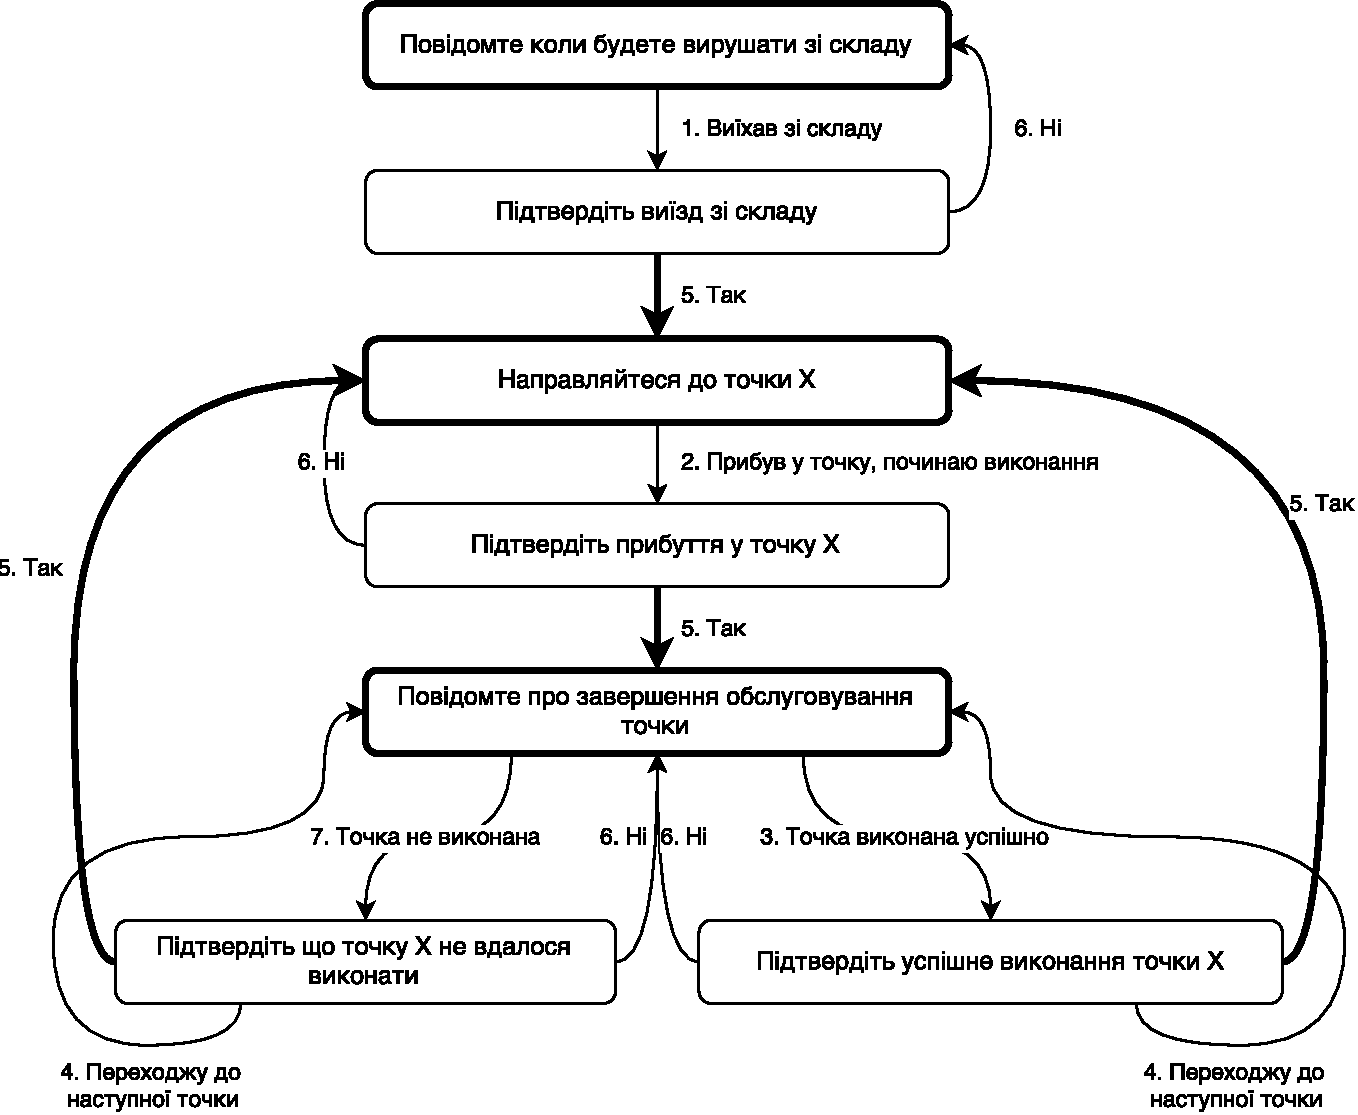
\includegraphics [width=1\linewidth] {05_simple_negative_scenario_with_conformation}
	\caption{Спрощений варіант дерева сценаріїв з негативними інцидентами}
	\label{img:05_simple_negative_scenario_with_conformation}
\end{figure}

Також у моделі голосової взаємодії водія в системах диспетчерського контролю за рухом автотранспорту може бути запропонований один з варіантів дерева сценаріїв з негативними інцидентами та відбоєм (рис. \ref{img:06_simple_negative_scenario_with_rollback}). Для наведеного випадку зʼявляється блок у дереві сценаріїв, повʼязаний з підтвердженням неприбуття на точку Х. Тобто в дереві сценаріїв зʼявляється звʼязок з відбоєм виконання та обслуговування точки Х при моделюванні голосової взаємодії водія в системах диспетчерського контролю за рухом автотранспорту. "Спрощений" варіант прибирає додаткове підтвердження для "переходжу до наступної точки". Щоб зберегти стійкість до помилок і простоту діалогу, замість підтвердження додаємо можливість відмінити цю останню дію.

\begin{figure}
	\centering
	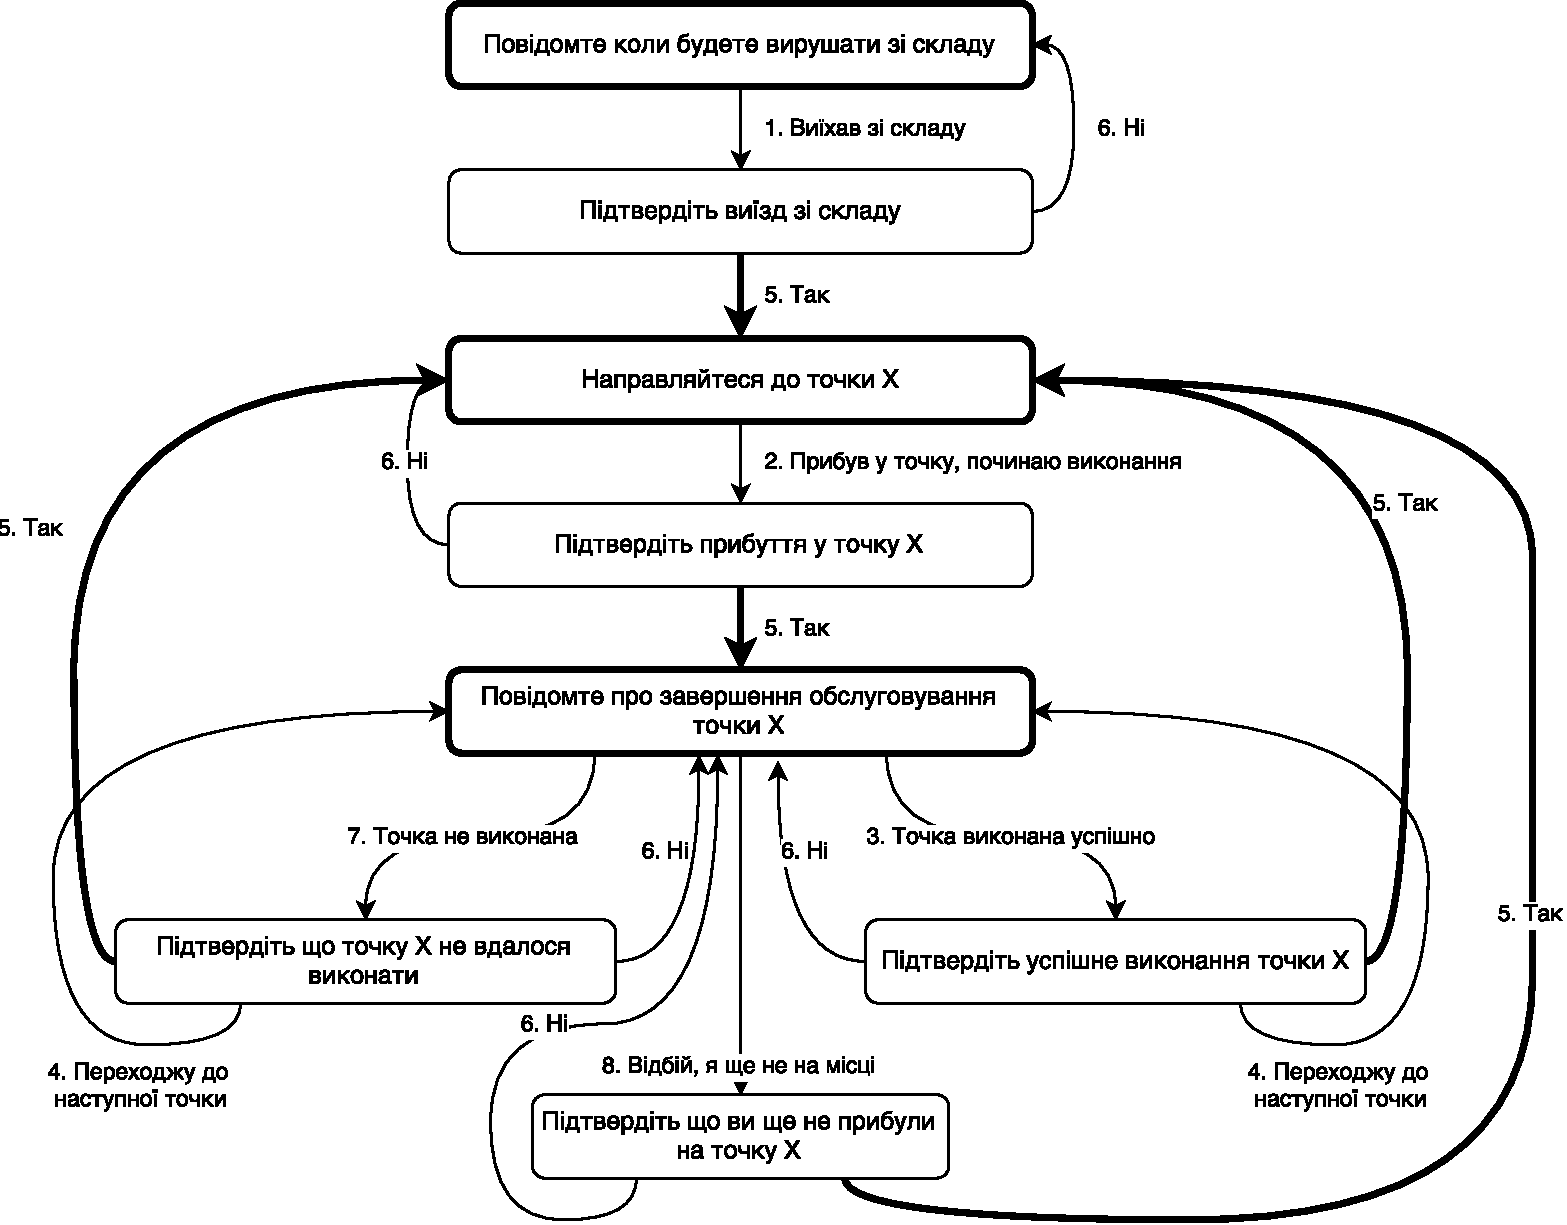
\includegraphics [width=1\linewidth] {06_simple_negative_scenario_with_rollback}
	\caption{Варіант дерева сценаріїв з негативними інцидентами та відбоєм}
	\label{img:06_simple_negative_scenario_with_rollback}
\end{figure}

Оскільки дерево стає занадто великим для зображення, для подальшої деталізації розбиваємо його на частини згідно до трьох основних етапів. Частина дерева сценаріїв етапу «точка доставки» у вертикальному розподілі приведена на рис. \ref{img:07_simple_point_scenario}, у горизонтальному – на рис. \ref{img:07_simple_point_scenario_horizontal}.
Приведені фрагменти дерева сценаріїв етапу «точка доставки» у вертикальному (рис. \ref{img:07_simple_point_scenario}) та горизонтальному (рис. \ref{img:07_simple_point_scenario_horizontal}) розподілах включають виконання та обслуговування попередньої точки Y, поточної точки Х та наступної Z, що розташовані на відповідних дорогах.

\begin{figure}
	\centering
	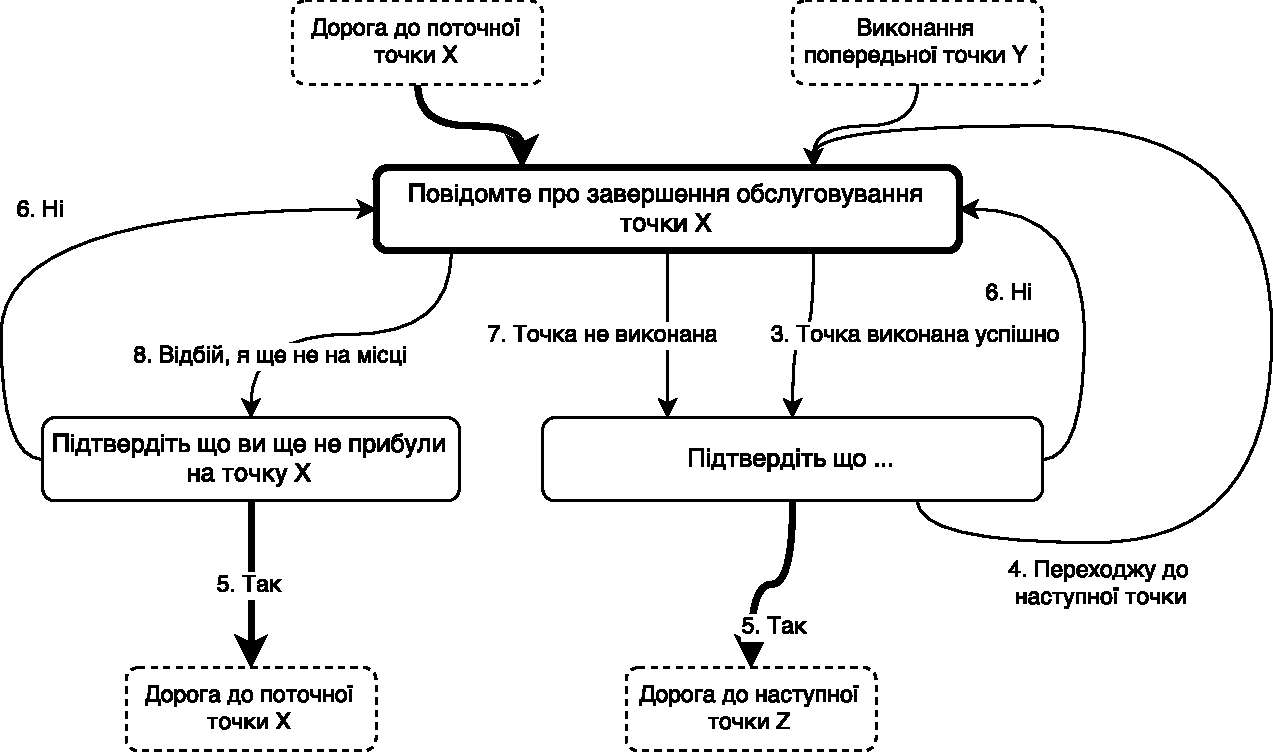
\includegraphics [width=1\linewidth] {07_simple_point_scenario}
	\caption{Частина дерева сценаріїв етапу <<точка доставки>>}
	\label{img:07_simple_point_scenario}
\end{figure}

\begin{figure}
	\centering
	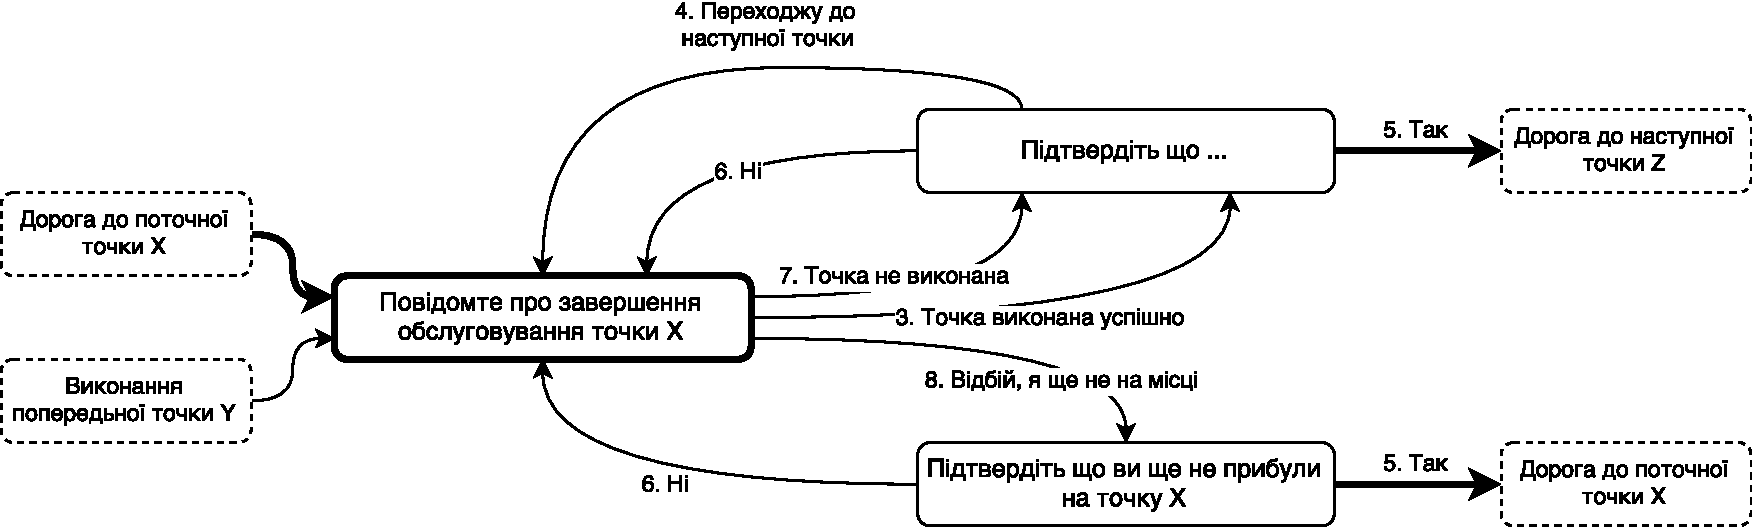
\includegraphics [width=1\linewidth] {07_simple_point_scenario_horizontal}
	\caption{Частина дерева сценаріїв етапу <<точка доставки>> в горизонтальному розподілі}
	\label{img:07_simple_point_scenario_horizontal}
\end{figure}

Як бачимо з рис. \ref{img:07_simple_point_scenario} та \ref{img:07_simple_point_scenario_horizontal}, горизонтальний розподіл є більш компактним.
На рис. \ref{img:08_complete_point_scenario} приведена одна з частин дерева сценаріїв етапу «точка доставки» з усіма негативними інцидентами при моделюванні голосової взаємодії водія в системах диспетчерського контролю за рухом автотранспорту.


\begin{figure}
	\centering
	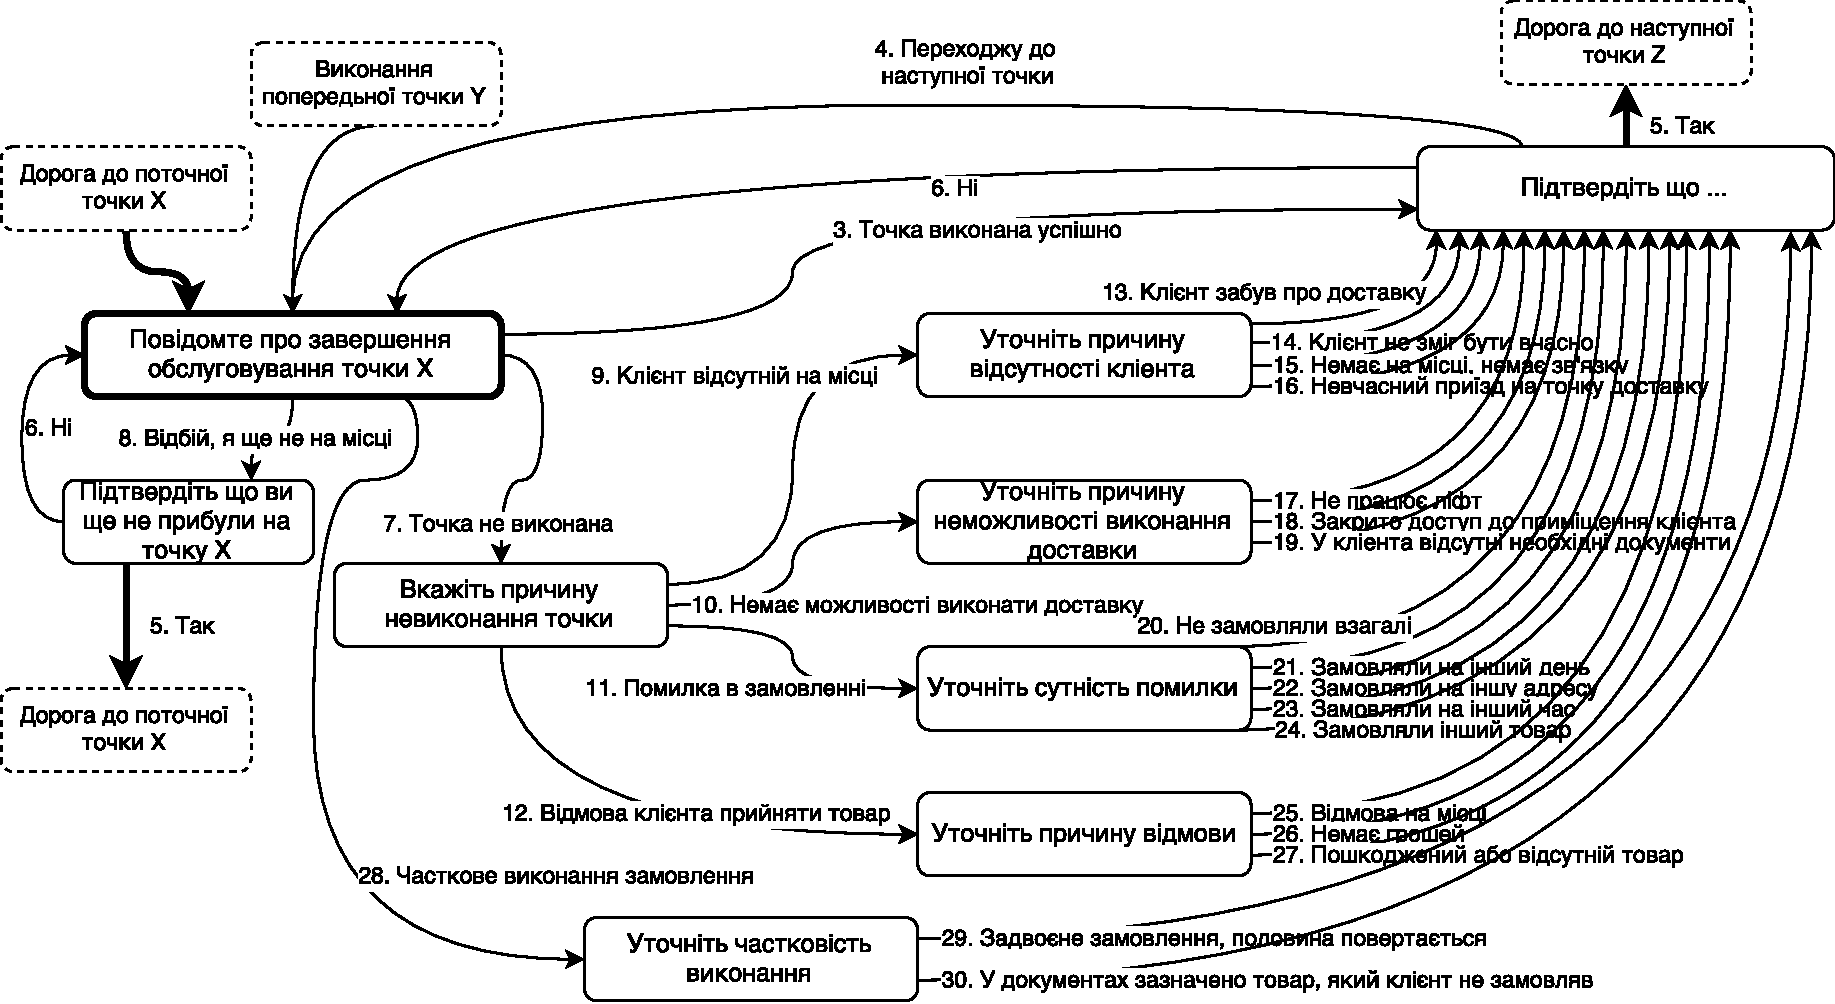
\includegraphics [width=1\linewidth] {08_complete_point_scenario}
	\caption{Частина дерева сценаріїв етапу <<точка доставки>> з усіма негативними інцидентами}
	\label{img:08_complete_point_scenario}
\end{figure}

Приведена частина дерева сценаріїв етапу «точка доставки» (рис. \ref{img:08_complete_point_scenario}) включає блок невиконання точки Х з розширеним уточненням причин та блок часткового виконання з характеристиками такого виконання.

На рис. \ref{img:08_complete_point_scenario_with_other} побудовано частину дерева сценаріїв етапу «точка доставки» з усіма негативними інцидентами та врахуванням деяких інших непередбачених подій невиконання точки Х з більш розширеним уточненням причин в порівнянні з деревом сценаріїв, що приведено на рис. \ref{img:08_complete_point_scenario} та частковим виконанням з більш розширеними характеристиками такого часткового виконання. Для зберігання відкритості досліджуваної системи на етапі моделювання не можуть бути враховані всі можливі варіанти розвитку подій, тому на рис. \ref{img:08_complete_point_scenario_with_other} приведені деякі непередбачувані події невиконання точки Х.

\begin{figure}
	\centering
	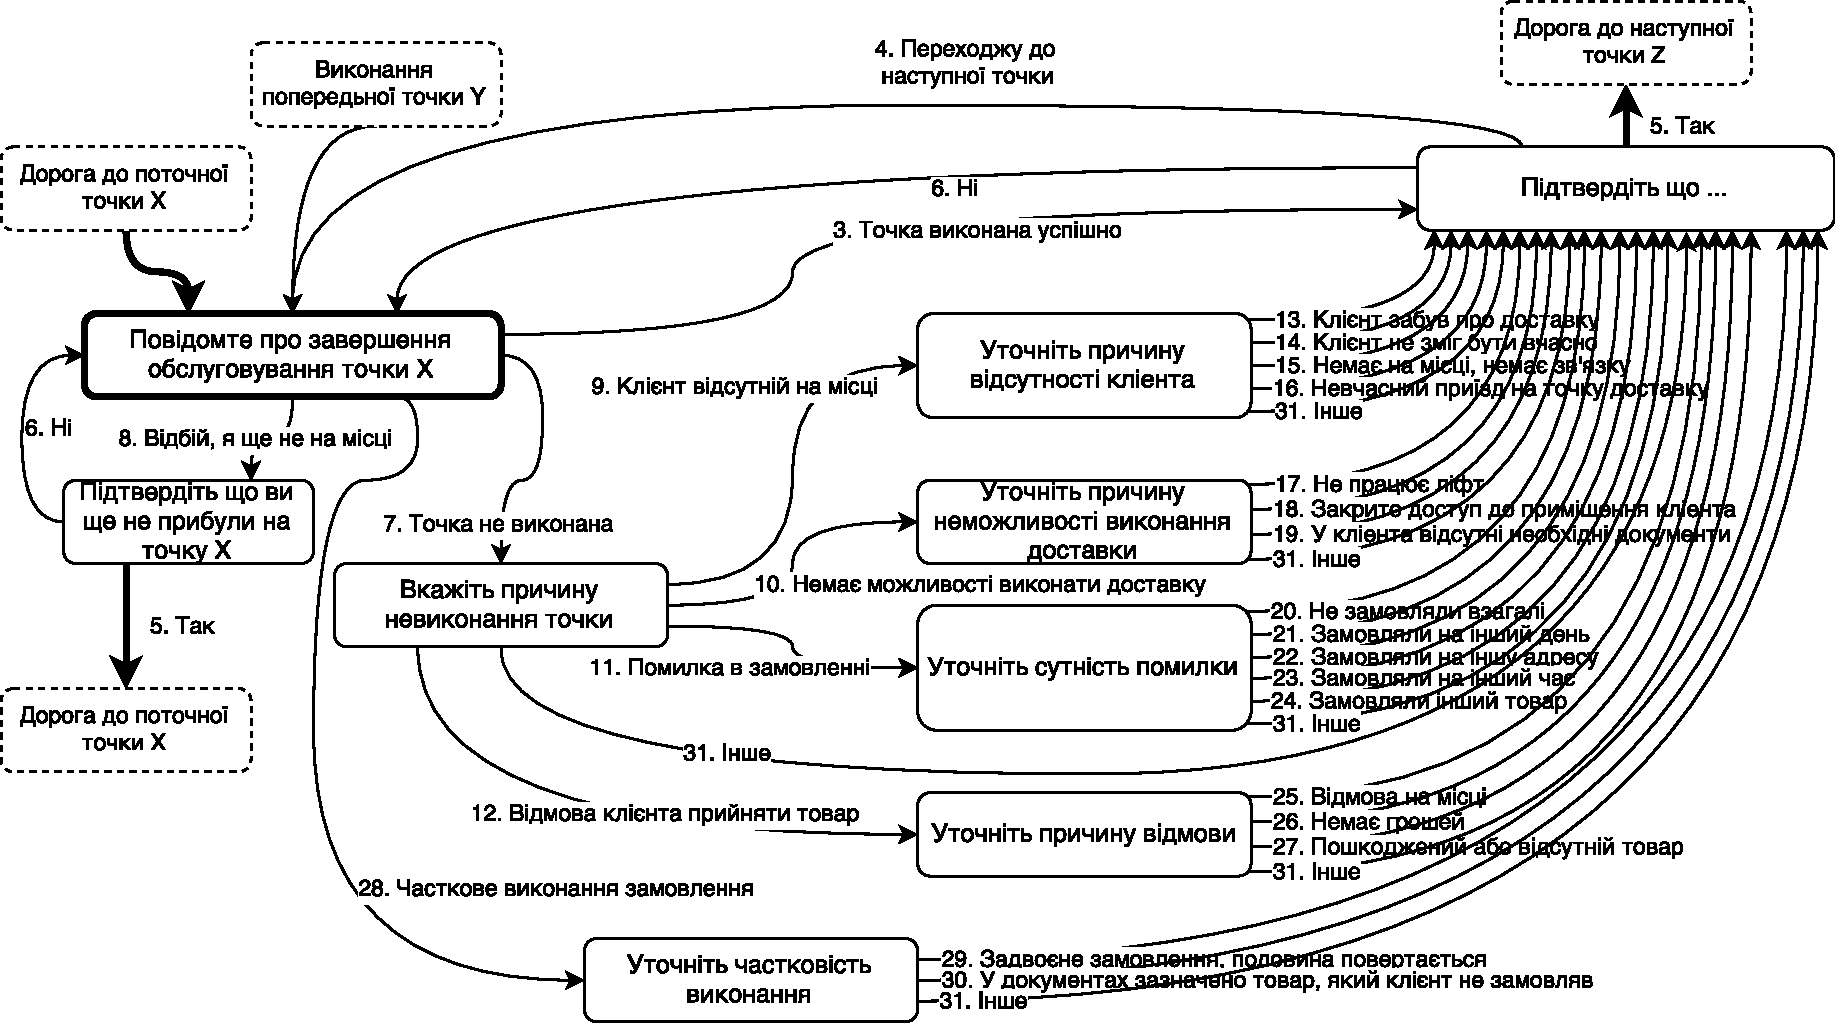
\includegraphics [width=1\linewidth] {08_complete_point_scenario_with_other}
	\caption{Частина дерева сценаріїв етапу <<точка доставки>> з усіма негативними інцидентами та урахуванням інших непередбачених подій}
	\label{img:08_complete_point_scenario_with_other}
\end{figure}

На рис. \ref{img:09_complete_point_scenario_with_rollback} приведена частина дерева сценаріїв етапу «точка доставки» з усіма негативними інцидентами та відбоєм із діалогового режиму. Можемо бачити, що для випадку відбою причин невиконання точки Х із діалогового режиму відбувається перехід до констатації обслуговування та успішного виконання точки Х при моделюванні голосової взаємодії водія в системах диспетчерського контролю за рухом автотранспорту.

\begin{figure} 
	\centering
	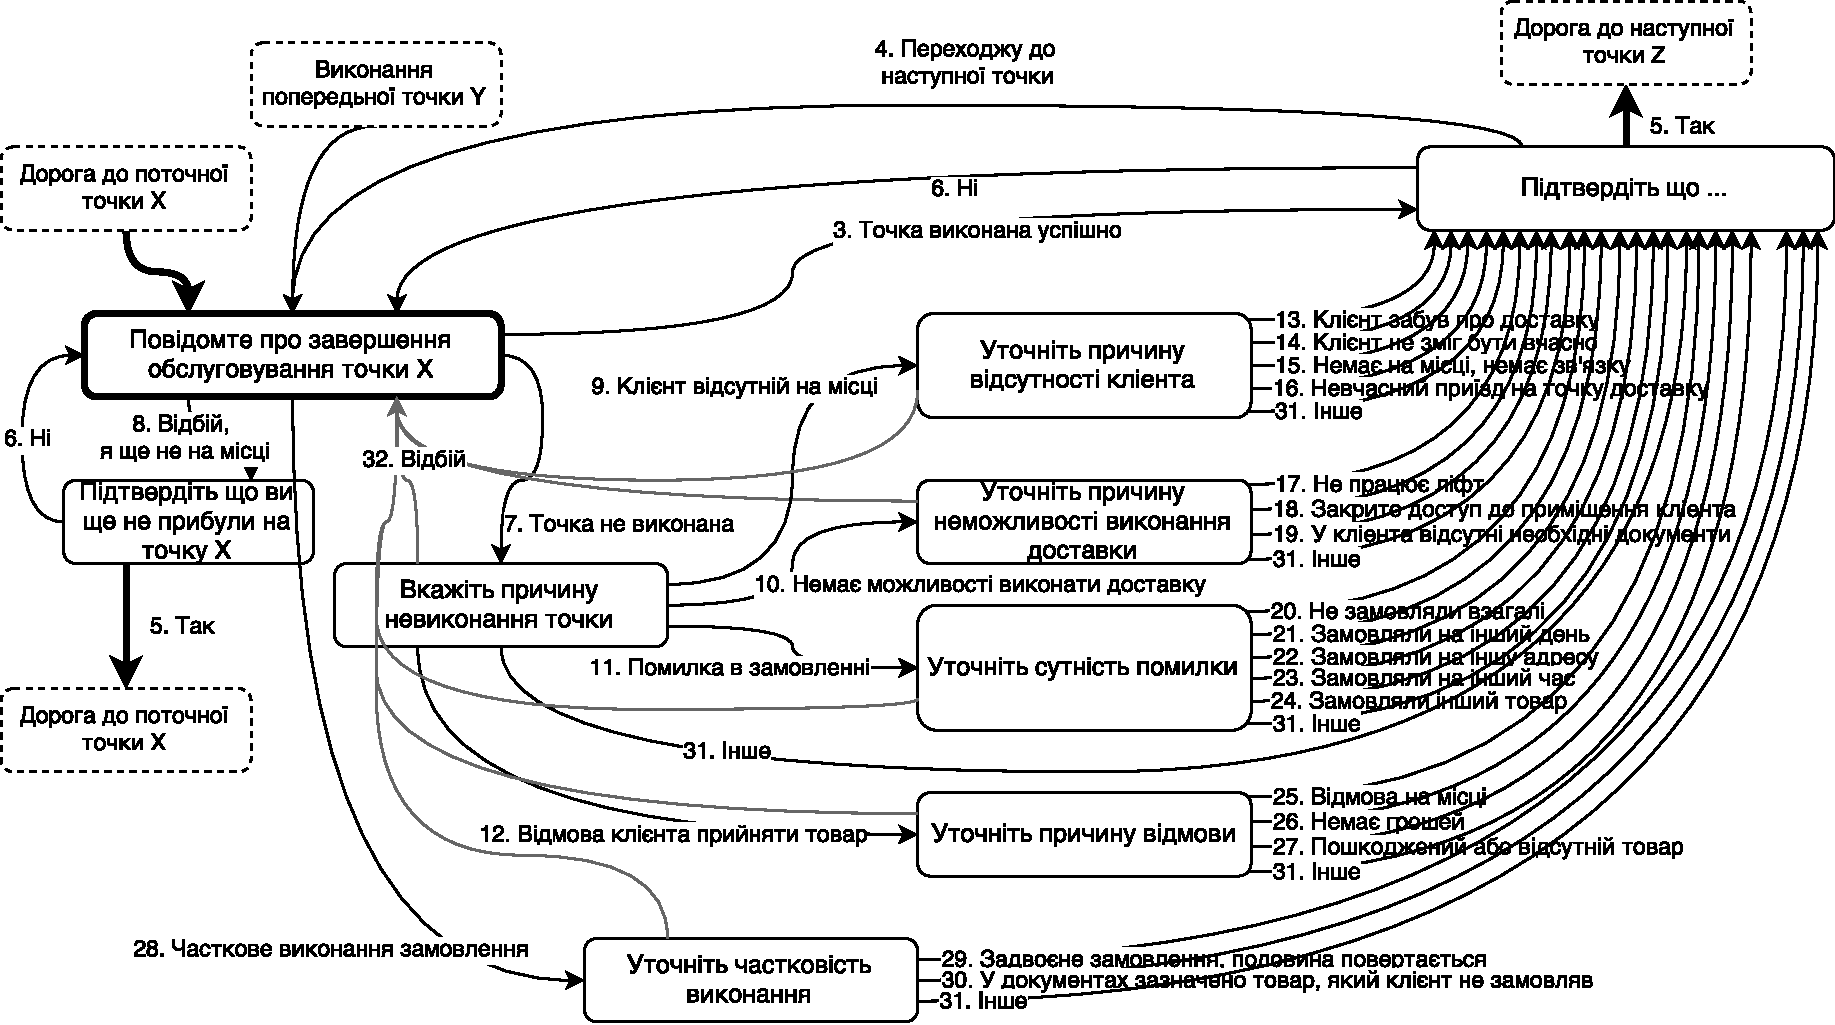
\includegraphics [width=1\linewidth] {09_complete_point_scenario_with_rollback}
	\caption{Частина дерева сценаріїв етапу "точка доставки" з усіма негативними інцидентами та відбоєм із діалогового режиму}
	\label{img:09_complete_point_scenario_with_rollback}
\end{figure}

Для випадку застосування додаткових функцій при моделюванні голосової взаємодії водія в системах диспетчерського контролю за рухом автотранспорту побудоване дерево сценаріїв етапу «точка доставки», частина якого приведена на рис. \ref{img:10_point_scenario_with_enchantment}.

\begin{figure}
	\centering
	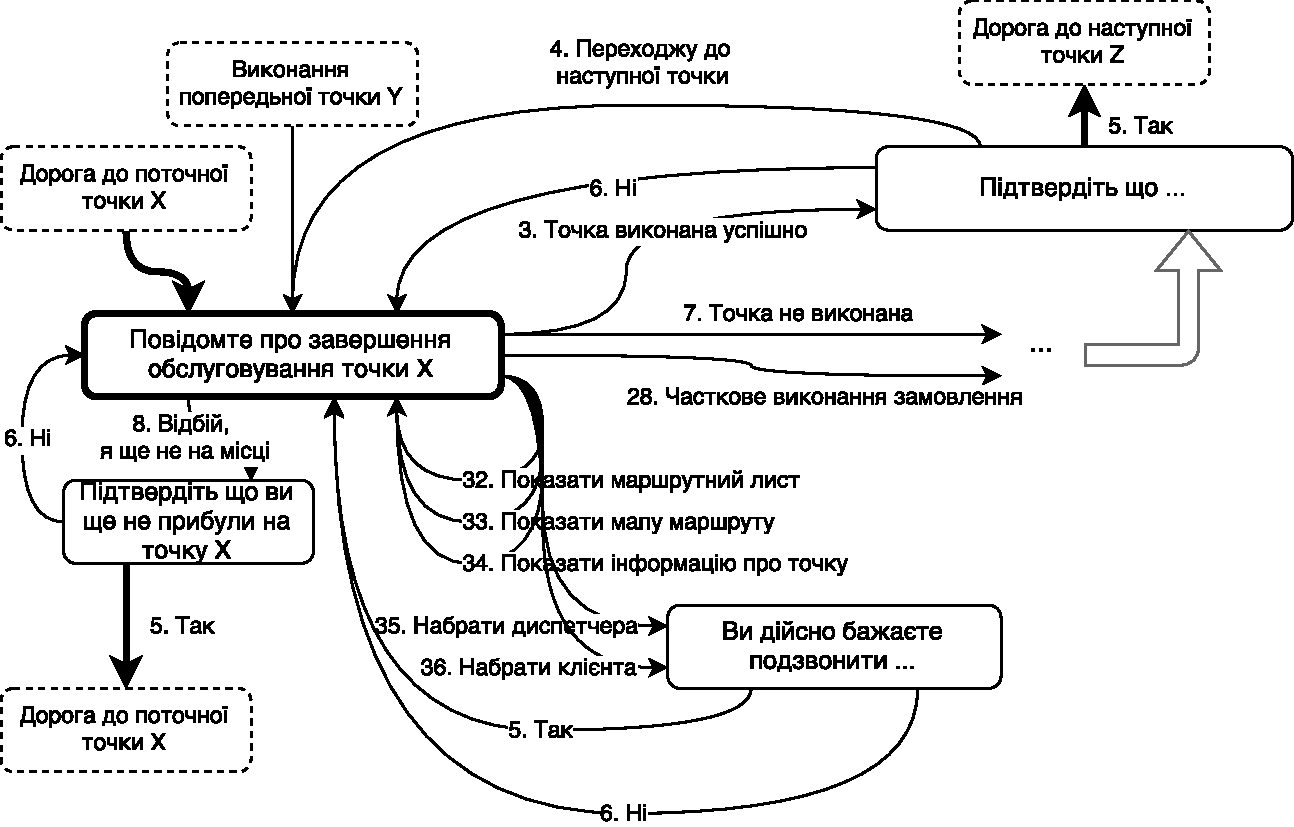
\includegraphics [width=1\linewidth] {10_point_scenario_with_enchantment}
	\caption{Частина дерева сценаріїв етапу <<точка доставки>> з додатковими функціями}
	\label{img:10_point_scenario_with_enchantment}
\end{figure}

У приведеній частині дерева сценаріїв етапу «точка доставки» (рис. \ref{img:10_point_scenario_with_enchantment}) присутні додаткові функції для водія при моделюванні його голосової взаємодії, повʼязані з інформаційними характеристиками маршруту до точки доставки Х, а також функції для набору диспетчера або клієнта.

На етапі «дорога» – дерево сценаріїв для моделі голосової взаємодії водія в системах диспетчерського контролю за рухом автотранспорту має наступний вигляд (рис. \ref{img:11_complete_road_scenario}). У наведеній частині дерева сценаріїв етапу «дорога» враховані всі контексти з репрезентативної вибірки даних, що отримані у ведучих логістичних компаніях України. При цьому, у випадку невиконання етапу «дорога» пропонуються причини затримки чи неможливості виконання маршруту з наступними інструкціями диспетчера, а у випадку, коли зʼявляється можливість виконання маршруту до точки доставки Х існує відбій із діалогового режиму.

\begin{figure}
	\centering
	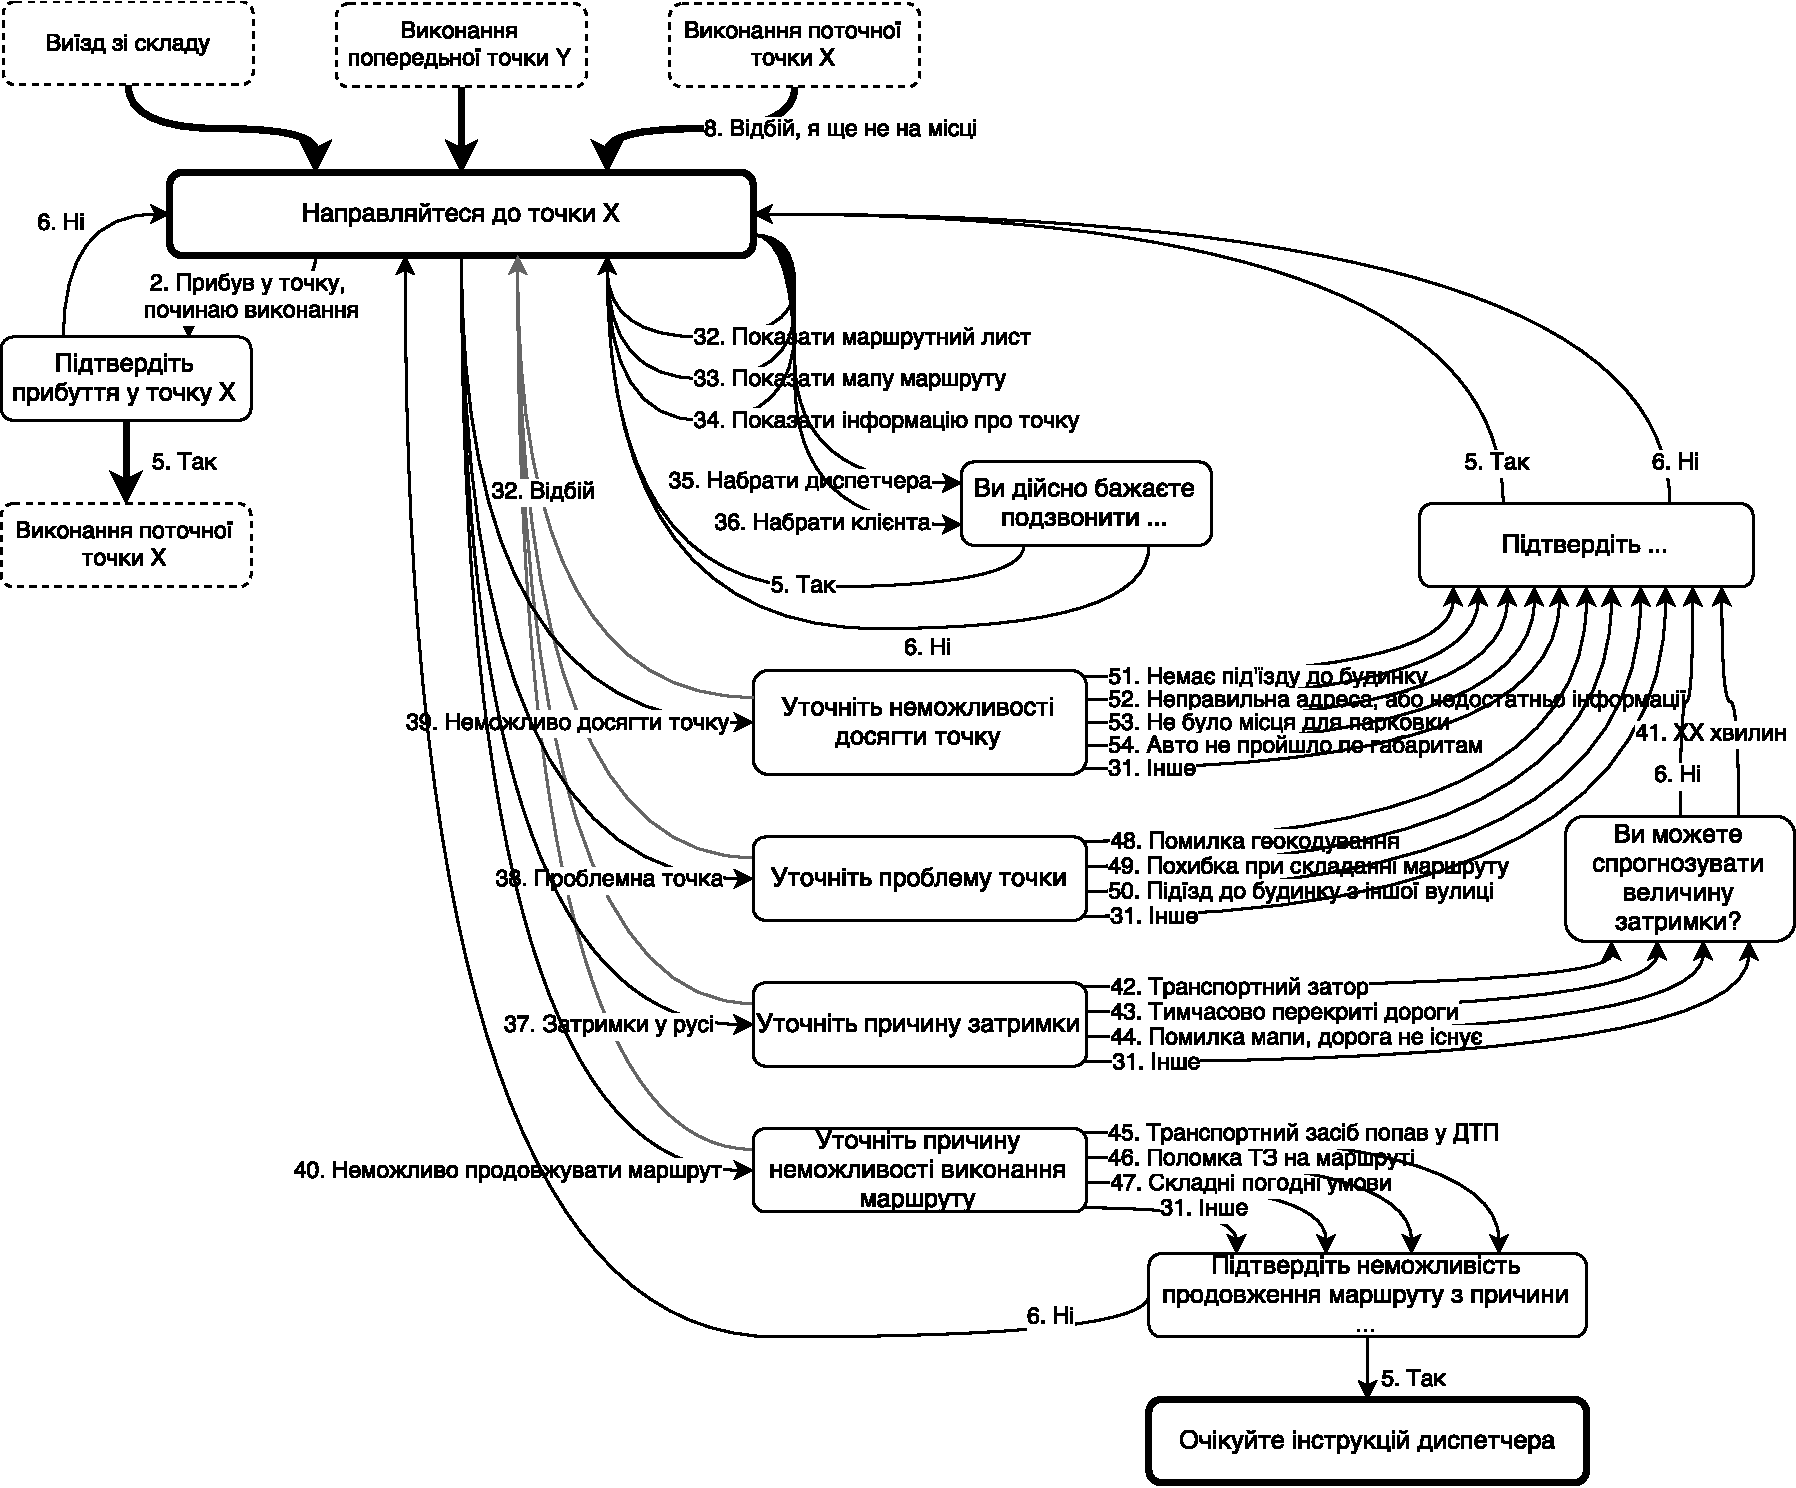
\includegraphics [width=.8\linewidth] {11_complete_road_scenario}
	\caption{Частина дерева сценаріїв етапу <<дорога>>}
	\label{img:11_complete_road_scenario}
\end{figure}

\begin{figure}
	\centering
	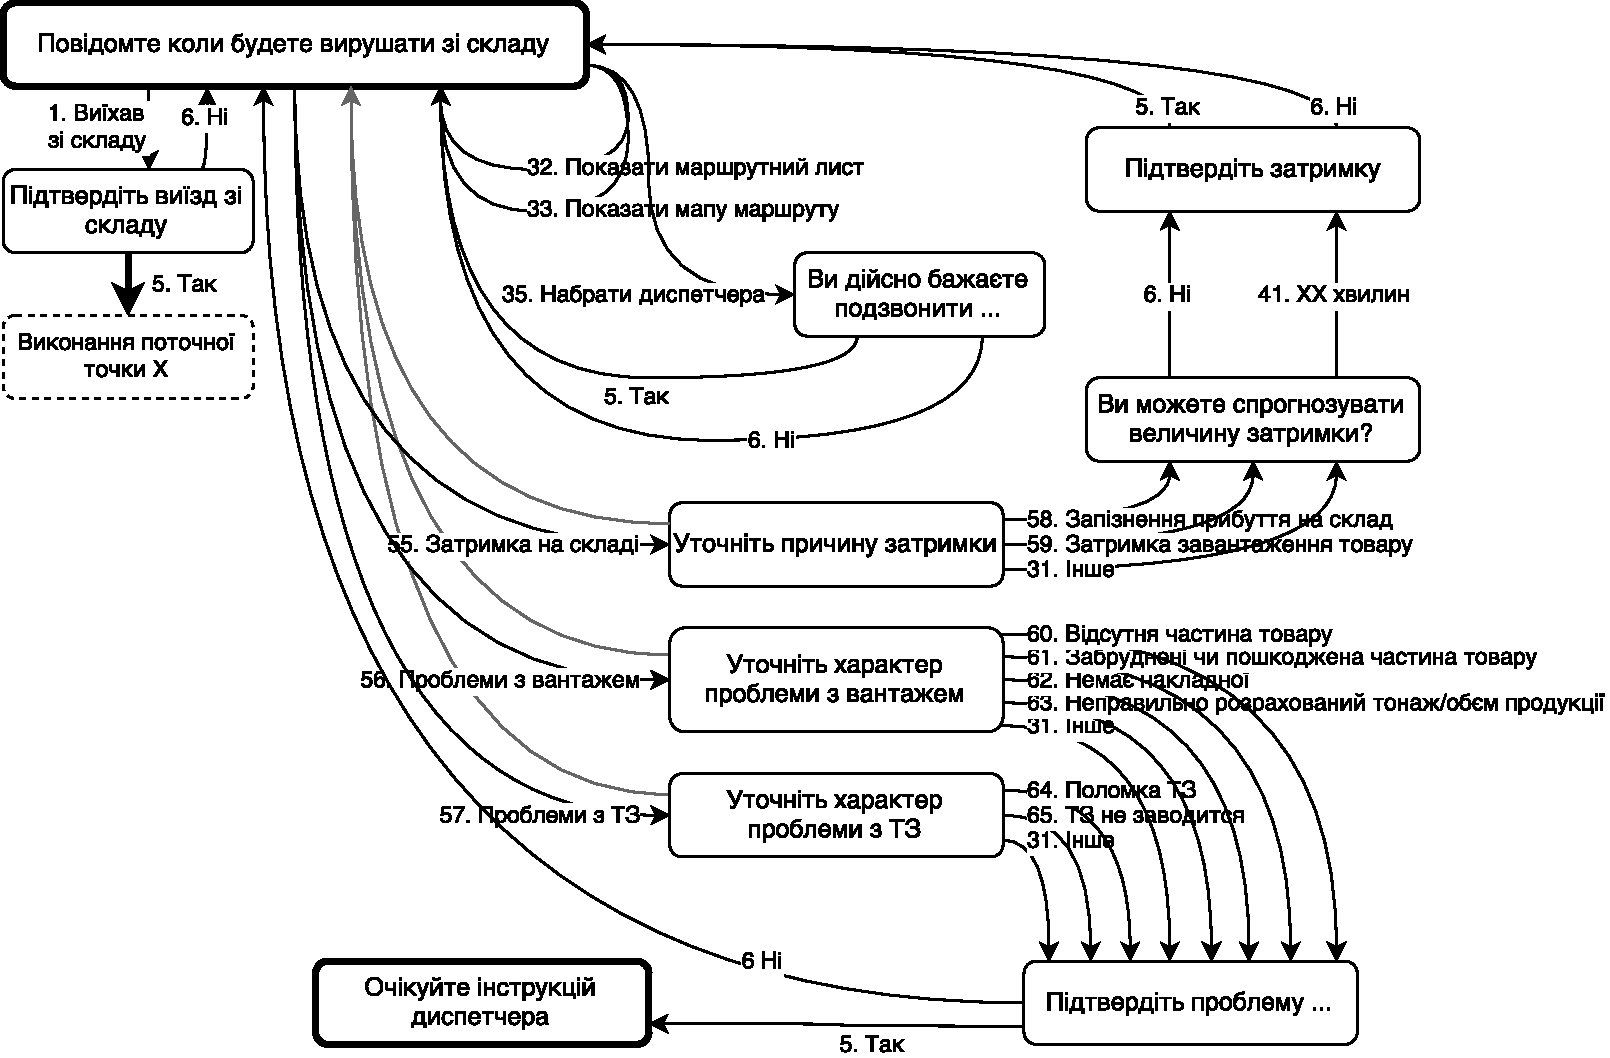
\includegraphics [width=.8\linewidth] {12_complete_depot_scenario}
	\caption{Частина дерева сценаріїв етапу <<склад>>}
	\label{img:12_complete_depot_scenario}
\end{figure}

Для виконання етапу «склад» субʼєктом дистрибуції – водієм при його голосовій взаємодії в системі диспетчерського контролю за рухом автотранспорту побудовано дерево сценаріїв етапу «склад», частина якого приведена на рис. \ref{img:12_complete_depot_scenario}.

В побудованому дереві сценаріїв етапу «склад» враховані негативні причини затримки чи невиїзду зі складу з можливістю отримати подальші інструкції диспетчера для вирішення проблеми.

Повне дерево сценаріїв усіх етапів дистрибуції «склад – дорога – точка доставки» в моделі голосової взаємодії водія в системі диспетчерського контролю за рухом автотранспорту наведено на рис. \ref{img:13_complete_scenario_graph}.

\begin{figure}
	\centering
	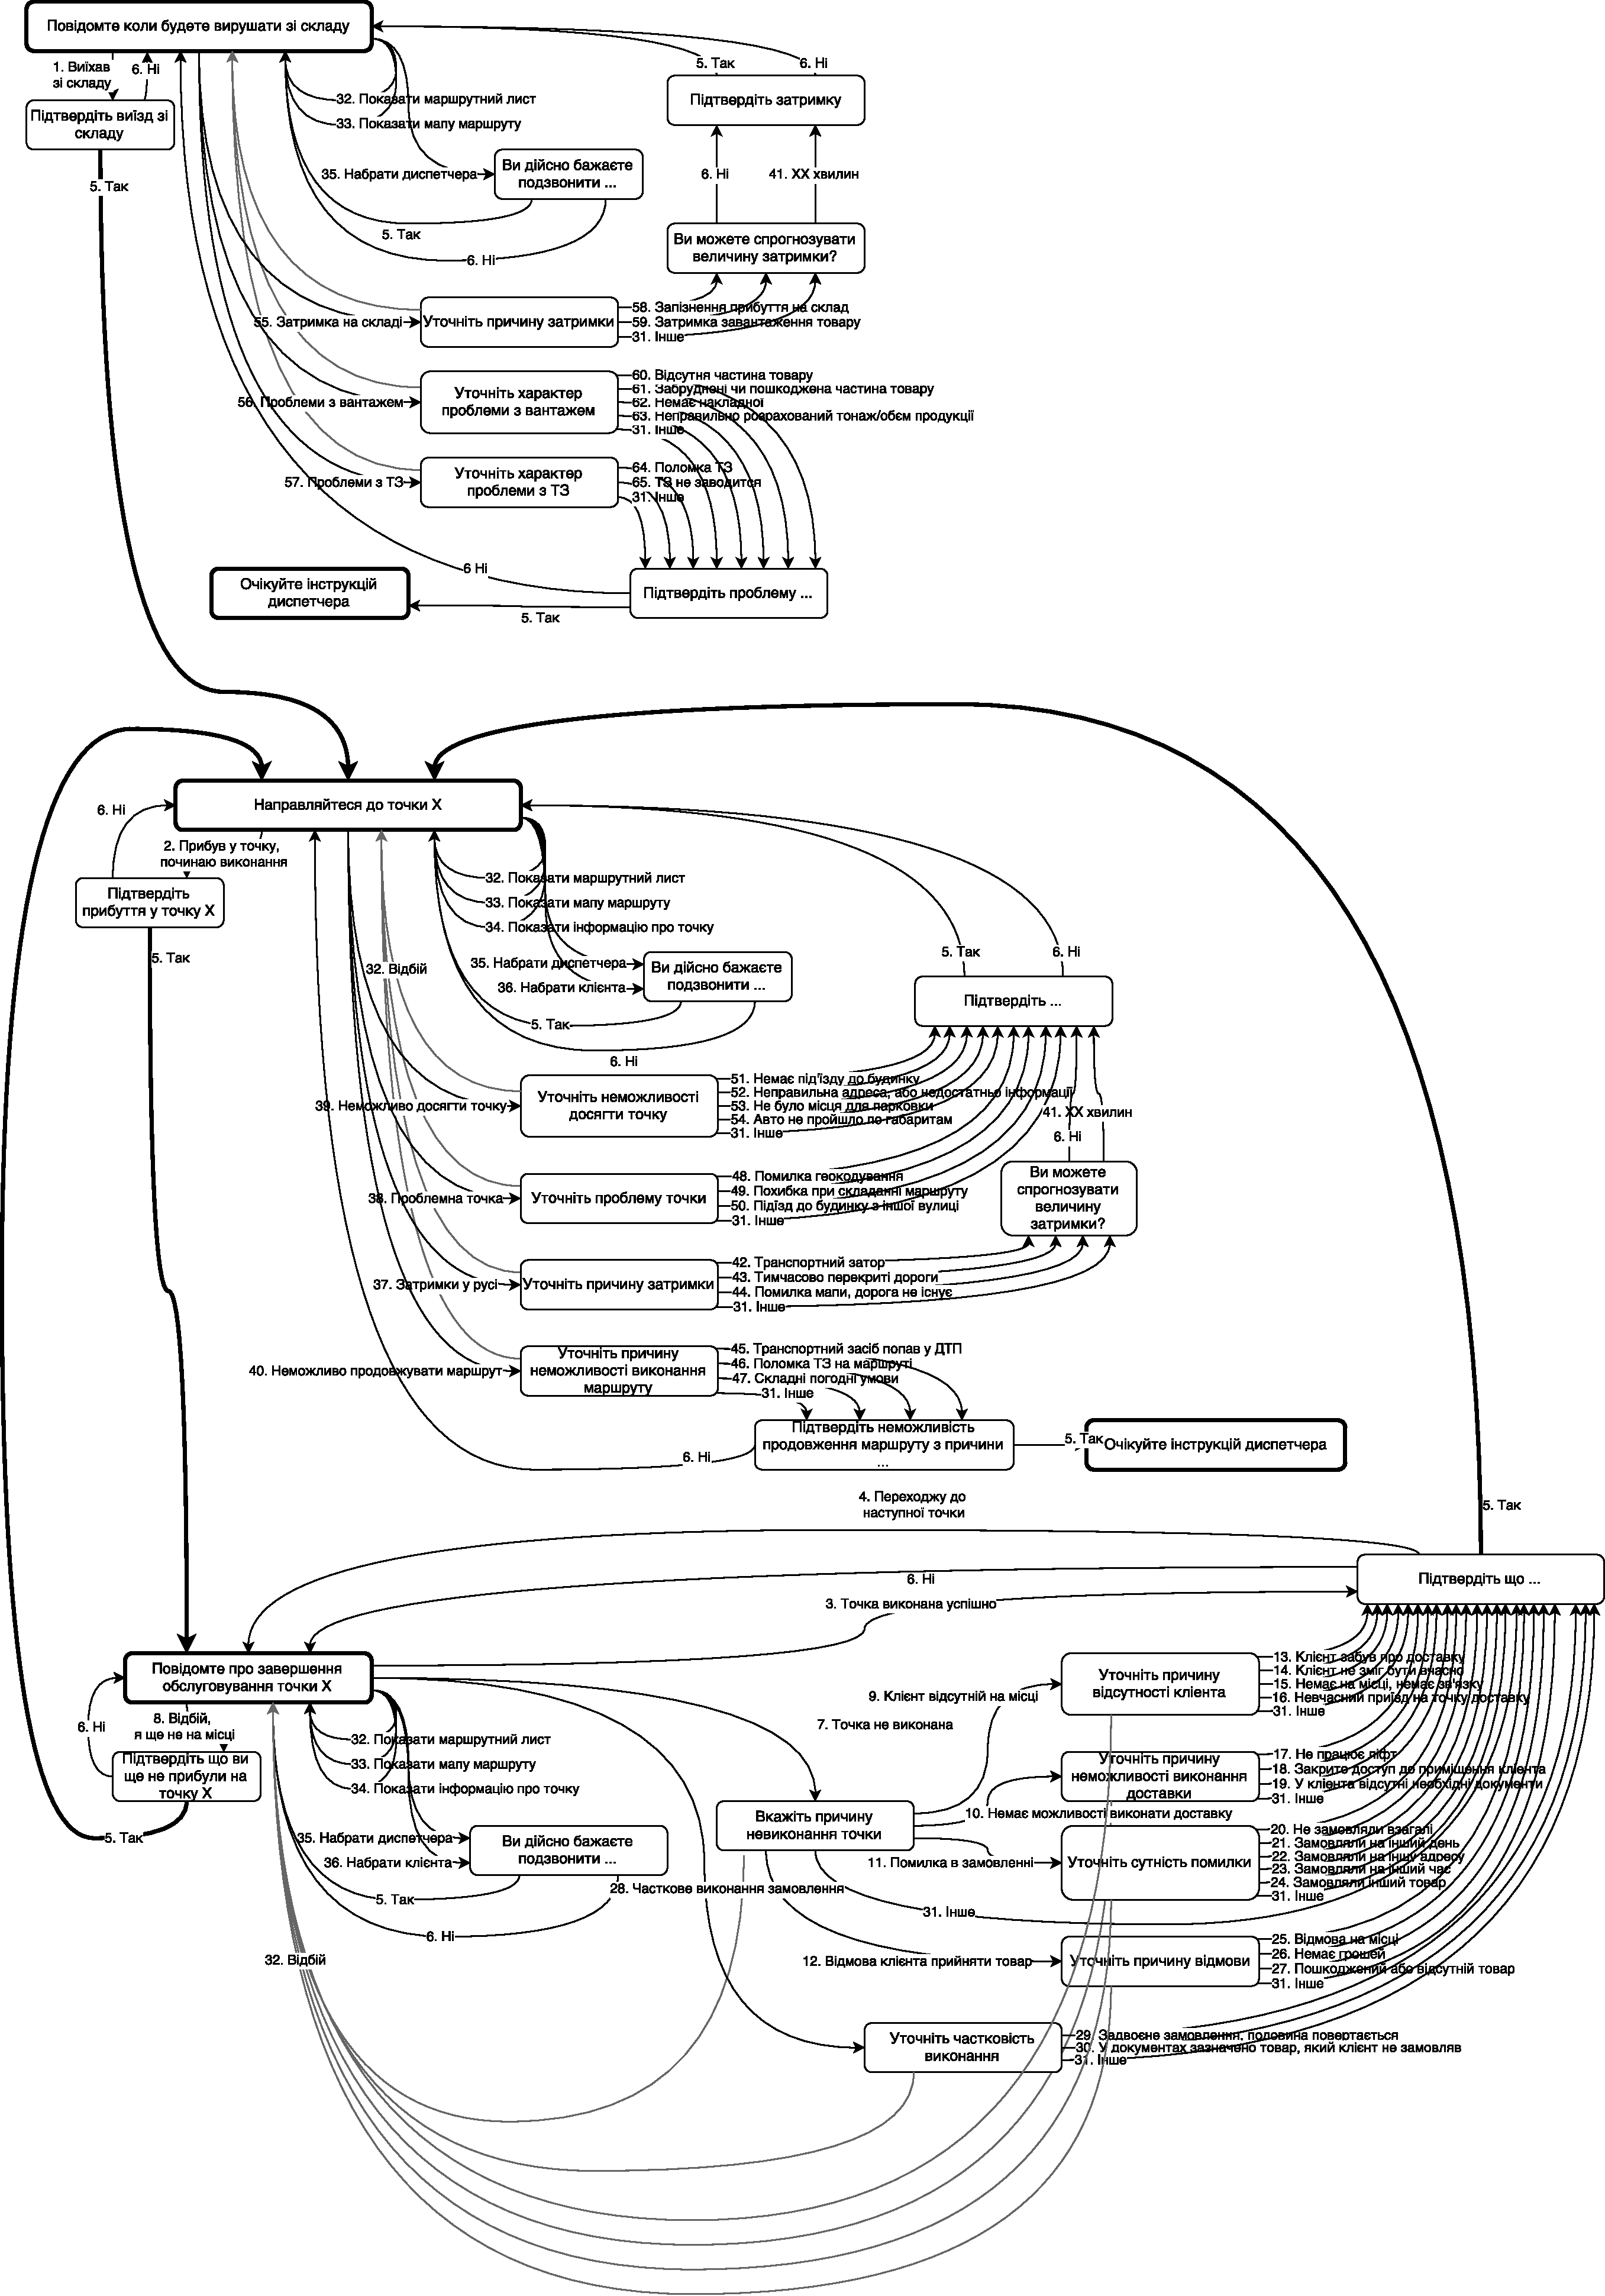
\includegraphics [width=1\linewidth] {13_complete_scenario_graph}
	\caption{Повне дерево сценаріїв всіх етапів}
	\label{img:13_complete_scenario_graph}
\end{figure}

\FloatBlock

В повному дереві сценаріїв усіх етапів дистрибуції (рис. \ref{img:13_complete_scenario_graph}) враховані всі можливі причини затримки або невиконання етапів «склад», «дорога», «точка доставки», а для таких випадків при неможливості виконання етапу існує вказівка (інструкції) диспетчера щодо подальших дій водія.

Приводимо повний перелік всіх унікальних стимулів з їх унікальними номерами в формі таблиці (табл. \ref{tbl:scenario_commands}).

\begin{mytable*}{ | c | l | }%
	{Різні варіанти стимулів з дерева сценаріїв}%
	{\label{tbl:scenario_commands}}%
	{№ & Варіанти стимулу}
	
	1 & Виїхав зі складу \\
	\hline
	2 & Прибув у точку, починаю виконання \\
	\hline
	3 & Точка виконана успішно \\
	\hline
	4 & Переходжу до наступної точки \\
	\hline
	5 & Так \\
	\hline
	6 & Ні \\
	\hline
	7 & Точка не виконана \\
	\hline
	8 & Відбій, я ще не на місці \\
	\hline
	9 & Клієнт відсутній на місці \\
	\hline
	10 & Немає можливості виконати доставку  \\
	\hline
	11 & Помилка в замовленні \\
	\hline
	12 & Відмова клієнта прийняти товар \\
	\hline
	13 & Клієнт забув про доставку \\
	\hline
	14 & Клієнт не зміг бути вчасно \\
	\hline
	15 & Немає на місці, немає звʼязку \\
	\hline
	16 & Невчасний приїзд на точку доставку \\
	\hline
	17 & Не працює ліфт \\
	\hline
	18 & Закрито доступ до приміщення клієнта \\
	\hline
	19 & У клиента відсутні необхідні документи \\
	\hline
	20 & Не замовляли взагалі \\
	\hline
	21 & Замовляли на інший день \\
	\hline
	22 & Замовляли на іншу адресу \\
	\hline
	23 & Замовляли на інший час \\
	\hline
	24 & Замовляли інший товар \\
	\hline
	25 & Відмова на місці \\
	\hline
	26 & Немає грошей \\
	\hline
	27 & Пошкоджений або відсутній товар \\
	\hline
	28 & Часткове виконання замовлення \\
	\hline
	29 & Задвоєне замовлення, половина повертається \\
	\hline
	30 & У документах зазначено товар, який клієнт не замовляв \\
	\hline
	31 & Інше \\
	\hline
	32 & Показати маршрутний лист \\
	\hline
	33 & Показати мапу маршруту \\
	\hline
	34 & Показати інформацію про точку \\
	\hline
	35 & Набрати диспетчера \\
	\hline
	36 & Набрати клієнта \\
	\hline
	37 & Затримки у русі \\
	\hline
	38 & Проблемна точка \\
	\hline
	39 & Неможливо досягти точку \\
	\hline
	40 & Неможливо продовжувати маршрут \\
	\hline
	41 & \# хвилин \\
	\hline
	42 & Транспортний затор \\
	\hline
	43 & Тимчасово перекриті дороги \\
	\hline
	44 & Помилка мапи, дорога не існує \\
	\hline
	45 & Транспортний засіб попав у ДТП \\
	\hline
	46 & Поломка ТЗ на маршруті \\
	\hline
	47 & Складні погодні умови \\
	\hline
	48 & Помилка геокодування \\
	\hline
	49 & Похибка при складанні маршруту \\
	\hline
	50 & Підʼїзд до будинку з іншої вулиці \\
	\hline
	51 & Немає підʼїзду до будинку \\
	\hline
	52 & Неправильна адреса, або недостатньо інформації \\
	\hline
	53 & Не було місця для парковки \\
	\hline
	54 & Авто не пройшло по габаритам \\
	\hline
	55 & Затримка на складі \\
	\hline
	56 & Проблеми з вантажем \\
	\hline
	57 & Проблеми з ТЗ \\
	\hline
	58 & Запізнення прибуття на склад \\
	\hline
	59 & Затримка завантаження товару \\
	\hline
	60 & Відсутня частина товару \\
	\hline
	61 & Забруднені чи пошкоджена частина товару \\
	\hline
	62 & Немає накладної \\
	\hline
	63 & Неправильно розрахований тоннаж/обʼєм продукції \\
	\hline
	64 & Поломка ТЗ \\
	\hline
	65 & ТЗ не заводится \\
\end{mytable*}%

Модель голосової взаємодії субʼєктів дистрибуції може бути представлена у вигляді орієнтовного графу $G$, що складається з множини вершин $V$ та множини ребер $E$:

\begin{align}
	G&=\langle V,E\rangle; \nonumber\\
	E&=\{\langle v_i,v_j\rangle | v \in V\}. \nonumber
\end{align}

При цьому існує відношення $f_R$ множини ребер на множину реакцій та відношення $f_C$ множини вершин на множину контекстів, такі що:

\begin{align}
	f_R&: E \rightarrow R,\quad R\subset\mathbb{N},\quad |R|\le|E|; \nonumber\\
	f_C&: V \rightarrow C,\quad C\subset\mathbb{N},\quad|C|\le|V|; \nonumber\\
	R_V(v_i) &= \{f_R(e)|\forall j:e=\langle v_i,v_j\rangle \in E\}; \nonumber\\
	\forall i,j: f_C(v_i)&=f_C(v_j) \iff R_V(v_i) = R_V(v_j), \nonumber
\end{align}

\noindent
де $R_V(v_i)$ множина реакцій можливих у вершині $v_i$.

Адекватність розробленої моделі підтверджується за рахунок того, що вона повністю відповідає статистичним даним інцидентів зібраних за період впровадження системи та експериментально, за рахунок порівняння результатів моделювання з використанням моделі, та без неї.

\subsection{Виділення унікальних контекстів моделі голосової взаємодії}

Як було зазначено в підрозділі \ref{sect2_3}, кожна вершина у орієнтованому графі сценаріїв голосової взаємодії водія в системах диспетчерського контролю за рухом автотранспорту (рис. \ref{img:13_complete_scenario_graph}) позначає контекст голосової взаємодії який може бути змодельовано окремо, а перелік ребер що виходять з цієї вершини, обмежує можливий перелік голосових команд, що мають  бути розпізнані в цьому контексті. 

Оскільки деякі контексти мають однаковий перелік можливих голосових команд, ми можемо не створювати для кожного з таких контекстів окрему модель, а повторно використовувати уже існуючі моделі контекстів з тим же переліком голосових команд. Для визначення переліку необхідних моделей, ми пронумеруємо всі контексти представлені на дереві сценаріїв в залежності від переліку команд які в них можуть бути розпізнані.

Повне дерево сценаріїв усіх етапів дистрибуції «склад – дорога – точка доставки» з вказівкою контекстів приведено на рис. \ref{img:14_complete_scenario_graph_contexts}. Використовуємо повне дерево сценаріїв, щоб знайти і пронумерувати унікальні контексти.

\begin{figure}
	\centering
	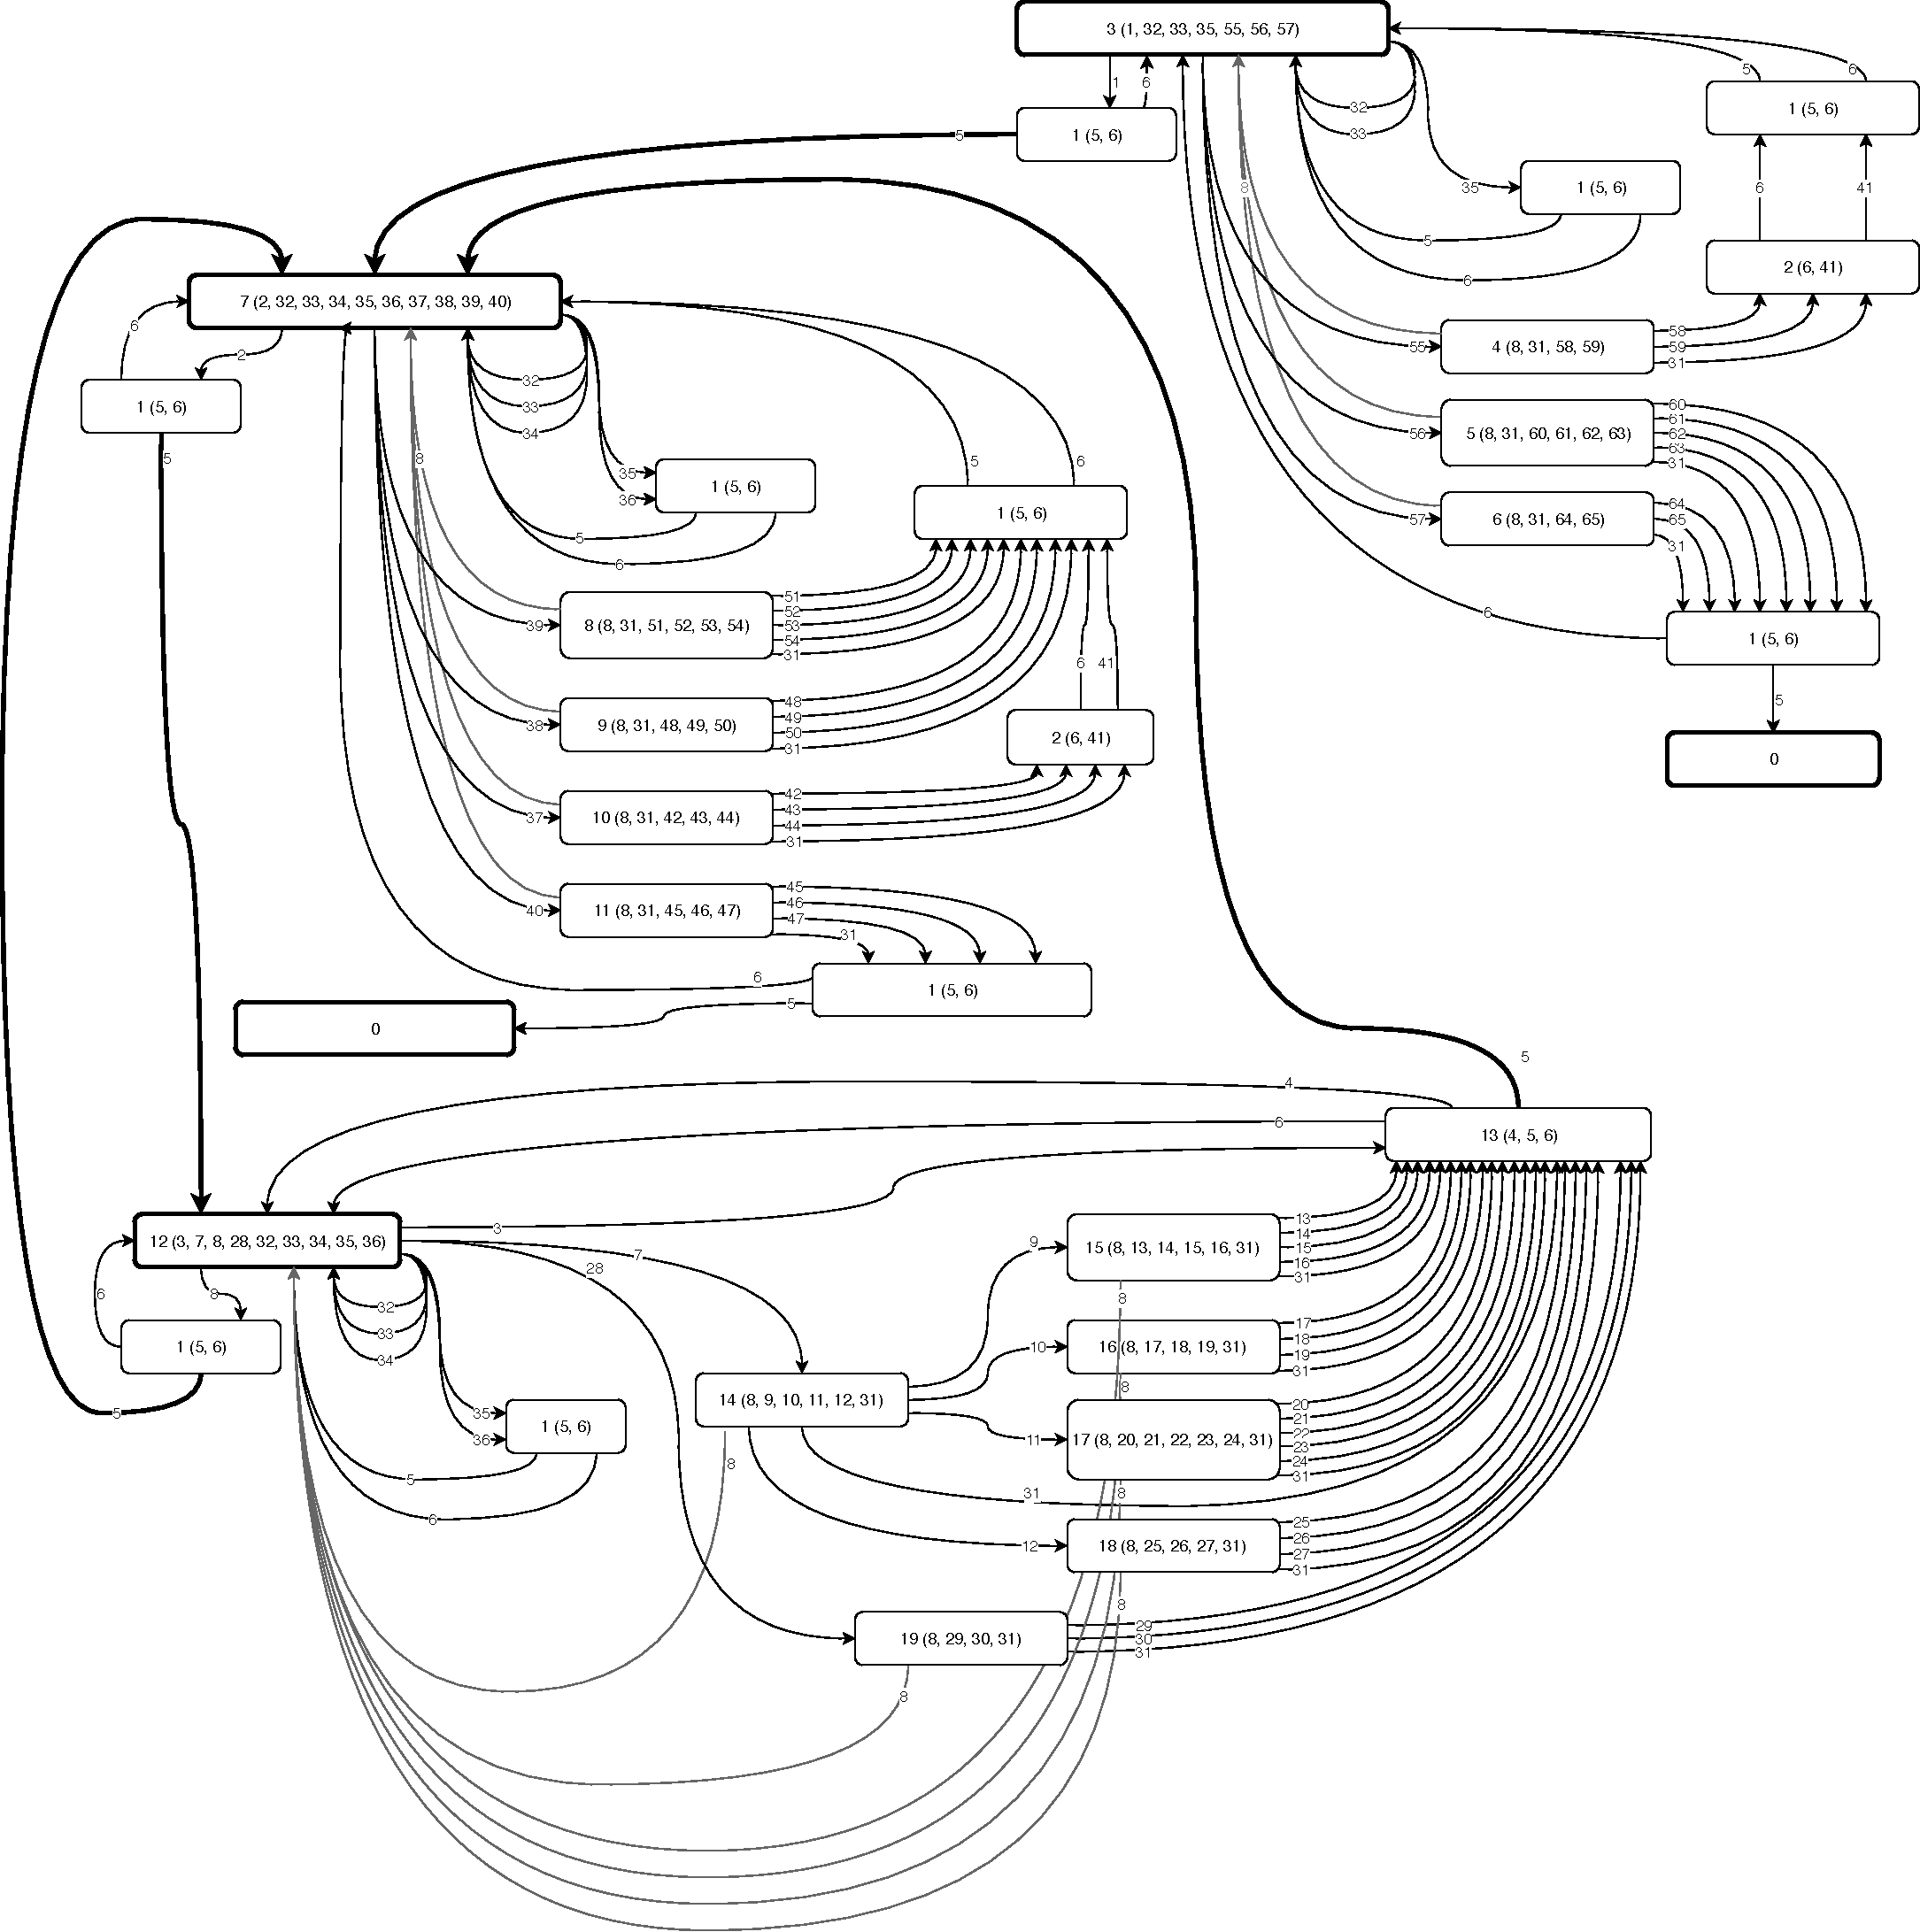
\includegraphics [width=1\linewidth] {14_complete_scenario_graph_contexts}
	\caption{Повне дерево сценаріїв всіх етапів з указанням контекстів}
	\label{img:14_complete_scenario_graph_contexts}
\end{figure}

Повне дерево сценаріїв всіх етапів дистрибуції «склад – дорога – точка доставки» з вказівкою контекстів (рис. \ref{img:14_complete_scenario_graph_contexts}) включає можливі реакції в них, тобто на кожний позначений контекст (табл. \ref{tbl:scenario_commands}) існує реакція, що вказана в дужках на дереві сценаріїв.

Приведемо в табл. \ref{tbl:context_reactions} звʼязок контекстів і реакцій на них в моделі голосової взаємодії водія в системі диспетчерського контролю за рухом автотранспорту.

Відповідно до приведених блоків контексту в моделі голосової взаємодії водія в системі диспетчерського контролю за рухом автотранспорту прослідковується звʼязок можливих реакцій на них, тобто відповідно до цього можна будувати систему формалізації голосової інформації.

\begin{mytable}{ | c | l | }%
	{Перелік контекстів та можливих реакцій у них}%
	{\label{tbl:context_reactions}}%
	{№ & Можливі реакції}
	
	1 & 5, 6 \\
	\hline
	2 & 6, 41 \\
	\hline
	3 & 1, 32, 33, 35, 55, 56, 57 \\
	\hline
	4 & 8, 31, 58, 59 \\
	\hline
	5 & 8, 31, 60, 61, 62, 63 \\
	\hline
	6 & 8, 31, 64, 65 \\
	\hline
	7 & 2, 32, 33, 34, 35, 36, 37, 38, 39, 40 \\
	\hline
	8 & 8, 31, 51, 52, 53, 54 \\
	\hline
	9 & 8, 31, 48, 49, 50 \\
	\hline
	10 & 8, 31, 42, 43, 44  \\
	\hline
	11 & 8, 31, 45, 46, 47 \\
	\hline
	12 & 3, 7, 8, 28, 32, 33, 34, 35, 36 \\
	\hline
	13 & 4, 5, 6 \\
	\hline
	14 & 8, 9, 10, 11, 12, 31 \\
	\hline
	15 & 8, 13, 14, 15, 16, 31 \\
	\hline
	16 & 8, 17, 18, 19, 31 \\
	\hline
	17 & 8, 20, 21, 22, 23, 24, 31 \\
	\hline
	18 & 8, 25, 26, 27, 31 \\
	\hline
	19 & 8, 29, 30, 31 \\
\end{mytable}%

\subsection{Створення моделі формалізації голосової інформації для кожного контексту голосової взаємодії}

Розглянемо будь-який контекст голосової взаємодії водія в системах диспетчеризації автотранспорту. Для формалізації голосової інформації в цьому контексті необхідно створити модель класифікації голосових висловлювань водія на класи відповідні до можливого переліку голосових команд у моделі голосової взаємодії.

Представимо перелік можливих голосових команд як множину:

\[
A = {A_i | i=\overline{1..n}},
\]

\noindent
де $A$ --- множина голосових команд $A_i$, а $n$ --- кількість можливих голосових команд в контексті, що розглядається.

Тоді для кожного голосового висловлювання $B$ сказаного водієм існує ймовірність $p(A_i/B)$, що це висловлювання було командою $A_i$. Задача формалізації голосової інформації полягає у визначенні яка з команд має найбільшу ймовірність.

Для вирішення цієї задачі пропонується дуальна система класифікації, яка може бути налаштована на предметну область і використовувати метод інтелектуальних рефлекторних систем чи метод згорткових нейронних мереж в залежності від того, який показує кращі результати. 

У даному підрозділі розроблено дерево сценаріїв усіх етапів дистрибуції «склад – дорога – точка доставки» як модель голосової взаємодії водія в системах диспетчерського контролю за рухом автотранспорту та визначено перелік контекстів та можливих реакцій на них.

\section{Дуальний метод формалізації голосової інформації в системах диспетчерського контролю за рухом автотранспорту} \label{sect3_4}

\subsection{Інтелектуальні рефлекторні системи}

Для формалізації голосової інформації можна використати систему з двох основних модулів: автоматичного фонетичного стенографа і ядра рефлекторної системи голосового управління (РСГУ), поточна реалізація яких визначає умови їх використання в моделі голосової взаємодії водія при диспетчерському контролі за рухом автотранспорту (рис. \ref{img:rsgu_struct}).

\begin{figure}
	\centering
	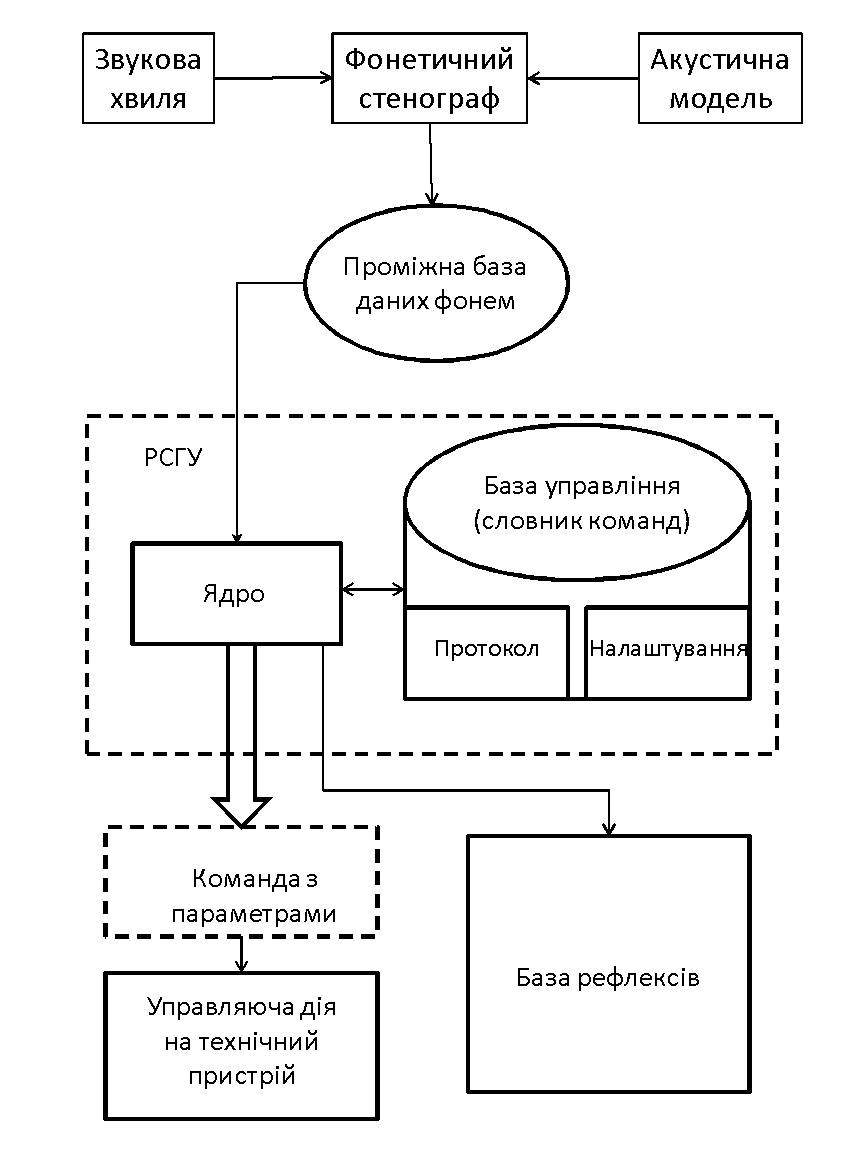
\includegraphics [width=.5\linewidth] {rsgu_struct}
	\caption{Структура системи формалізації голосової інформації в моделі голосової взаємодії водія при диспетчерському контролі за рухом автотранспорту}
	\label{img:rsgu_struct}
\end{figure}

Застосування алгоритму фонетичного стенографа дозволяє будувати послідовність контекстів для мовного сигналу без використання будь-якого словника. Для цієї мети будується деяка генеративна граматика, яка може синтезувати всі можливі модельні сигнали безперервної мови для будь-якої послідовності фонем. В рамках побудованої моделі будується алгоритм пофонемного розпiзнавання для невідомого сигналу з використанням контекстів та можливих реакцій на них.

Виконання фонетичного стенографу \cite{Pylypenko_2008} здійснено у вигляді бінарного додатку, набору бібліотек і конфігураційних файлів для платформи Windows, а саме ядро РСГУ виконує реалізацію інтроформаційного методу вироблення рефлексів, яке розроблено і виконано в середовищі MS Access на всіх операційних системах сімейства Windows.

У розглядаємій системі формалізації голосової інформації (рис. \ref{img:rsgu_struct}) вхідною інформацією виступає голосова команда, яка може бути представлена звуковою хвилею; вихідною ж інформацією буде виступати процес керуючого впливу на обʼєкт управління, тобто відбуватиметься виконання розпізнаної команди відповідно до попередньо заданих голосом параметрам.

Сама система формалізації голосової інформації в процесі роботи буде генерувати потрібні візуальні і голосові інформаційні повідомлення водію, це, в свою чергу, надає можливість відслідковувати процес розпізнавання команд, реакції на них і, крім того, дозволяє в реальному масштабі часу змінювати поведінку системи в разі потреби.

Розглянемо схему роботи системи формалізації голосової інформації в моделі голосової взаємодії водія при диспетчерському контролі за рухом автотранспорту. Водій у вільній формі озвучує необхідні для нього дії системи. Наприклад, по відношенню до голосового управління системою: «Показати маршрутний лист», або «Показати мапу маршруту», або «Показати інформацію про точку». Програмна платформа системи формалізації голосової інформації в моделі голосової взаємодії водія при диспетчерському контролі за рухом автотранспорту передає необхідну команду на технічний пристрій, або озвучує водієві інформацію, затребувану в його команді. При навчанні водій сам виконує відповідну дію, і у системи виробляється рефлекс на подібне звернення. Якщо водій (чи інший водій, який закріплений на автотранспортному засобі) говорить «по-різному», то виробляється стійкий рефлекс саме на інформативну частину голосової команди.

При цьому в системі формалізації голосової інформації в моделі голосової взаємодії водія при диспетчерському контролі за рухом автотранспорту наявні наступні стани, команди та засоби:

1. \textbf{Звукова команда}. Водій голосом звертається з проханням до технічного пристрою.

Вихідною інформацією є звукова хвиля.

Наведемо приклад для даної команди: покажи мені, будь ласка, інформацію про точку;

2. \textbf{Акустична модель}. Включає статистичний опис розпізнавання мови і особливостей мови водія. Статистичний опис формується в процесі навчання налаштуванням на водіїв. У якості акустичних моделей використовуються приховані Марківські моделі. 65 українських контекстно-незалежних фонем моделюються трьома станами Марківського ланцюга без пропуску.

Створення словника транскрипцій акустичних моделей відбувається автоматично з орфографічного словника з використанням контекстно-незалежних правил;

3. \textbf{Фонетичний стенограф}. Служить для перетворення вхідного оцифрованого звукового сигналу, що містить усне мовлення (акустичної моделі), в набір фонем.

Алгоритм фонетичного стенографа дозволяє будувати послідовність фонем для мовного сигналу без використання будь-якого словника. Для цієї мети будується деяка генеративна граматика, яка може синтезувати всі можливі модельні сигнали безперервної мови для будь-якої послідовності фонем. В рамках побудованої моделі будується алгоритм пофонемного розпiзнавання для невідомого сигналу. Використовуються ті ж контекстно незалежні моделі фонем, як і в базовому розпізнавачі.

Надійність виявлення фонеми на правильному місці для відомої реалізації дорівнює приблизно 70%.

Вихідна інформація: проміжна база даних фонем – результат розпізнавання вхідних звукових хвиль;

4. \textbf{Ядро РСГУ}. Призначено для моделювання системи голосового управління технічним пристроєм. Містить програмну реалізацію інтроформаційного методу, а також алгоритмів виділення комбінацій фонем і навчання (накопичення статистики). Інформаційна база управління містить словник команд, протокол роботи, налаштування системи;

5. \textbf{Команда з параметрами}. Результатом її роботи є команда з параметрами, яку необхідно реалізувати технічному пристрої.

Вихідною інформацією є виконувана команда.

Приклад: водій – Найдьонов, команда – Х хвилин, рівень – десятки, десятки хвилин – 10, одиниці хвилин – 8;

6. \textbf{Керуючий вплив}. Містить програмну реалізацію алгоритму управління технічним пристроєм.

Вхідною інформацією є перетворена у вигляд формули, команда з відповідними параметрами.

Результатом керуючого впливу є зміна параметрів самого технічного пристрою.

Прикладом керуючого пристрою може бути інформація про наступний час виконання.

Система формалізації голосової інформації в моделі голосової взаємодії водія при диспетчерському контролі за рухом автотранспорту є простою і, у даному випадку, реалізує рефлекторну модель поведінки, що приведена на рис. \ref{img:rsgu_scheme}

\begin{figure}
	\centering
	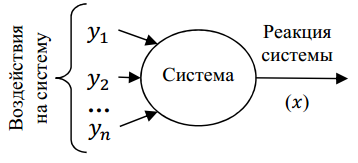
\includegraphics [width=.5\linewidth] {rsgu_scheme}
	\caption{Схема реакції системи формалізації голосової інформації в моделі голосової взаємодії водія при диспетчерському контролі за рухом автотранспорту на несилові впливи}
	\label{img:rsgu_scheme}
\end{figure}

Система формалізації голосової інформації в моделі голосової взаємодії водія при диспетчерському контролі за рухом автотранспорту функціонує в режимі навчання і режимі управління. У першому випадку у режимі навчання відбувається формування бази рефлексів.
У режимі управління РСГУ відбувається вироблення реакції на звернення водія. Також у цьому режимі відбувається реалізація режиму самонавчання – для випадку, коли отримана реакція не задовольняє водія.

Основною частиною системи формалізації голосової інформації в моделі голосової взаємодії водія при диспетчерському контролі за рухом автотранспорту є база рефлексів. База рефлексів містить статистику вхідних впливів (комбінацій фонем) і реакцій системи, розділених на класи: водій, команда, рівень числа, десятки, одиниці (рис. \ref{img:rsgu_base}).

\begin{figure}
	\centering
	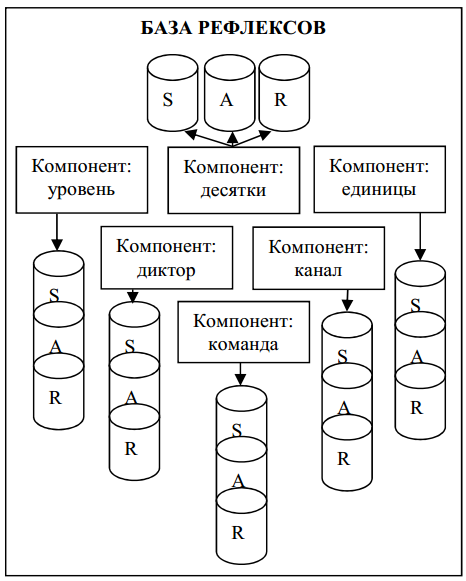
\includegraphics [width=.5\linewidth] {rsgu_base}
	\caption{Структура бази рефлексів системи формалізації голосової інформації}
	\label{img:rsgu_base}
\end{figure}

Реалізація кожного класу рефлексів відбувається в кожному окремому компоненті системи формалізації голосової інформації в моделі голосової взаємодії водія при диспетчерському контролі за рухом автотранспорту. Представлення кожного компоненту системи здійснюється у вигляді окремого «інтроформаційного» нейрона.

На вході системи задається повний вхідний набір фонем, та/або реакція інших «інтроформаційних» нейронів, на виході – вироблена реакція нейронів, яка надходить на інші «інтроформаційні» нейрони, або на самий технічний пристрій.

У кожному компоненті системи формалізації голосової інформації в моделі голосової взаємодії водія при диспетчерському контролі за рухом автотранспорту інформація зберігається в наступних таблицях:

\begin{itemize}
	\item S – таблиця з комбінацією фонем, в якій знаходяться та зберігаються всі комбінації послідовних фонем з довжинами від 2-х до 10 символів з інформацією про те, скільки разів вони зустрічалися;
	\item R – таблиця реакції РСГУ, в якій міститься перелік дій, що необхідно виконати РСГУ або технічному пристрою, частота користування і визначеність даної реакції. Реакція типу «Не знаю» забезпечує відкритість системи;
	\item А – таблиця, що призначена для встановлення звʼязку вищенаведених таблиць S і R. Дана таблиця вміщує інформацію про те, скільки разів і яка реакція була затребувана в разі, коли на вході був деякий набір фонем. Крім того, дана таблиця містить відомості про визначеність реакції, що повʼязана з цим набором фонем.
\end{itemize}

У вищенаведених таблицях для випадку режиму навчання відбувається накопичення інформації про звʼязок вхідних фраз (контекстів) і реакцій системи формалізації голосової інформації в моделі голосової взаємодії водія при диспетчерському контролі за рухом автотранспорту. У процесі роботи системи отримана інформація використовується далі в режимі управління для вироблення реакцій на відповідні звернення водія на основі інтроформаційного методу \cite{Teslia_2010}. При цьому алгоритм реалізації режиму управління в системі має наступну послідовність:

\begin{itemize}
	\item перший етап. Старт алгоритму.
\end{itemize}

При надходженні на вхід системи потоку фонем виділяються фрагменти (набори), множиною M, що містять від 2 до 4 поруч стоячих символів;

\begin{itemize}
	\item другий етап. Відбір класу команд.
\end{itemize}

З таблиці S відбувається здійснення відбору записів, які відповідають сформованим наборам фонем, що належать до множини M.
На основі інтроформаційного методу відбувається обчислення визначеності реакцій (команд), що містяться в таблицях A і R. Команда, що має найбільшу визначеність, вибирається для реалізації;

\begin{itemize}
	\item третій етап. Якщо в команді є звернення до числового значення (знак \#), розглядаються класи рівень числа, десятки, одиниці.
\end{itemize}

Клас рівня числа. У таблиці S здійснюється відбір записів, які відповідають сформованим наборам фонем (що входять у множину M). Використовуючи таблиці A і R, відповідно до інтроформаційного методу обчислюється визначеність рівня числа. Варіанти: немає десятків хвилин (числа від 0 до 9), є десятки хвилин (числа більше 9).

Якщо рівень числа «Є десятки хвилин», то активізуються таблиці, що входять в клас десятків хвилин. У таблиці S здійснюється відбір записів, які відповідають сформованим наборам фонем (що входять в множину M). Використовуючи таблиці A і R, відповідно до інтроформаційного методу обчислюється визначеність номера десятка. Якщо десяток не визначений, в команду вставляється знак «?».

Клас одиниць хвилин. У таблиці S здійснюється відбір записів, які відповідають сформованим наборам фонем (що входять в множину M). Використовуючи таблиці A і R, відповідно до інтроформаційного методу обчислюється визначеність другий цифри в числі. Якщо цифра не визначена, в команду вставляється знак «?»;

\begin{itemize}
	\item четвертий етап. Завершення алгоритму.
\end{itemize}

Отже метод інтелектуальних рефлекторних систем для формалізації голосової інформації в системах диспетчерського контролю за рухом автотранспорту можна представити наступним чином:

\begin{enumerate}
	\item запис фрази вимовленої водієм; $A_i=<a_1,a_2,...,a_n>; t=\frac{n}{s}; s=16 \textbf{(kHz)};$
	\item перетворення записаної фрази на фонетичний текст, за допомогою фонемного стенографа; $P_i=S(A_i); P=<p_1,p_2,...,p_k>; p_i \in F;$
	\item класифікація фонемної репрезентації голосової команди; $y_i=C_c(P_i)$
	\begin{enumerate}
		\item розбиття фонетичного тексту на N-грами фонем різної довжини;
		\item розрахунок інтроформаційного впливу кожного N-граму фонем на можливі команди в вибраному контексті;
		\item вибір команди з найбільшою ймовірністю;
	\end{enumerate}
	\item виконання відповідної реакції (озвучення відповіді, виконання команди та/або відправка структурованих даних диспетчеру);
	\item переключення контексту на новий, відповідний до вибраної реакції; $c_{i+1} = f(c_i, y_i)$
	\item очікування та запис наступної фрази.
\end{enumerate}

{\settowidth{\leftskip}{Де:\ }
	
	$A_i$ --- цифровий аудіозапис команди водія довжиною $t$ секунд,
	
	$n$ --- кількість семплів аудіо сигналу,
	
	$s$ --- частота дискретизації аудіо сигналу,
	
	$P_i$ --- представлення команди водія у вигляді фонемного тексту --- кортежу фонем довжини $k$,
	
	$F$ --- множина фонем української мови,
	
	$S$ --- фонемний стенограф,
	
	$y_i$ --- реакція з моделі голосової взаємодії субʼєктів дистрибуції що відповідає вимовленій команді,
	
	$C_c$ --- класифікатор фонемної репрезентації голосових команд відповідно до поточного контексту $c_i$
	
	$f$ --- функція визначення наступного контексту в залежності від поточного контексту $c_i$ та вибраної реакції $y_i$
	
}

Таким чином, в кожен компонент системи надходить весь вхідний набір фонем. Без виділення слів, команд, пропозицій тощо. Результат даного методу такий самий як і у головного мозку людини. Тобто, слухаючи усне мовлення, або читаючи лист, мозок, не розпізнаючи букви і слова, розпізнає сенс. Теж саме відбувається і в рефлекторній системі голосового управління. При цьому, не потрібно створювати ніяких словників, виконувати морфологічний, синтаксичний, семантичний аналіз тексту, а також виділяти слова і команди; виникнення реакції відбувається на звуковий потік, з якого система формалізації голосової інформації в моделі голосової взаємодії водія при диспетчерському контролі за рухом автотранспорту, як і людина сама «вміє виділяти» інформативну частину за максимальною визначеністю \cite{Teslia_2013}.

Для покращення ефективності розпізнавання була запропонована удосконалена схема системи формалізації голосової інформації в моделі голосової взаємодії водія в дистрибуції (рис. \ref{img:rsgu_struct_new}), яка включає моделювання за кожним контекстом із моделі голосової взаємодії та дуальну систему класифікації фонемної репрезентації голосових команд, що дозволяє вибрати кращий метод класификації в залежності від предметної області.

\begin{figure}[h!]
	\centering
	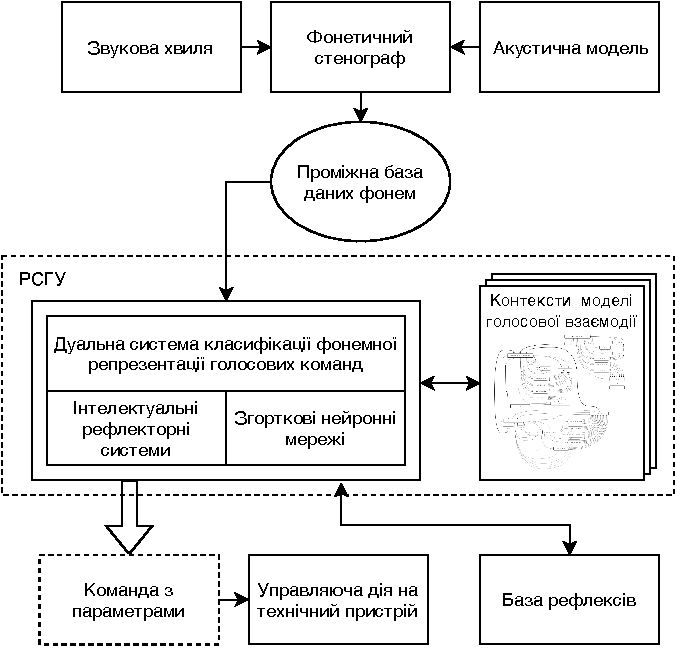
\includegraphics [width=.6\linewidth] {rsgu_struct_new}
	\caption{Удосконалена схема системи формалізації голосової інформації в моделі голосової взаємодії водія при диспетчерському контролі за рухом автотранспорту}
	\label{img:rsgu_struct_new}
\end{figure}

У якості альтернативного класифікатора фонетичного тексту голосової команди запропоновано використання методу згорткових нейронних мереж, що широко використовується в різноманітно задачах класифікації звукових даних \cite{Weisskirchen_2017,Boddapati_2017,Chowdhury_2018} та природномовних текстів \cite{Kim_2014,Britz_2015_2,Britz_2015,Kim_2016,Zhang_2015_2,Zhang_2015,Santos_2014}.

\subsection{Згорткові нейронні мережі}

У даному випадку система формалізації голосової інформації в моделі голосової взаємодії водія при диспетчерському контролі за рухом автотранспорту аналогічно до РСГУ, складається з двох частин: фонемний стенограф та сама згорткова нейронна мережа (ЗНМ), яка працює з фонемами.
ЗНМ для роботи з фонемами найбільше нагадує ЗНМ в задачі класифікації текстів \cite{Kim_2014}, але оперує з «текстом» не по словах, а пофонемно, що схоже на роботу з текстом посимвольно \cite{Zhang_2015}.

ЗНМ дуже схожі на звичайні нейронні мережі: вони також побудовані на основі нейронів, які володіють постійно змінюваною вагою і зсувами. Кожен нейрон отримує деякі вхідні дані, виконує скалярне перетворення інформації і, в окремих ситуаціях, супроводжується нелінійністю. Як і у випадку зі звичайними нейронними мережами, вся ЗНМ висловлює одну диференційовану функцію внеску (ефективний внесок): з одного боку це необроблені фонеми, з іншого – висновок класу або групи ймовірних класів, які характеризують фонему. Також присутня функція втрати на останньому (повністю підключеному) шарі ЗНМ.

Архітектура ЗНМ робить явне припущення виду «вхідні дані є фонеми», що дозволяє закодувати певні властивості під архітектуру. Завдяки цій особливості, попереднє оголошення можна реалізувати більш ефективно, зменшуючи при цьому кількість параметрів в мережі.

Як відомо, нейронні мережі отримують вхідні дані (один вектор), після чого трансформують інформацію, проводячи її через ряд прихованих шарів \cite{Kim_2014, Zhang_2015}. Кожен прихований шар складається з безлічі нейронів, де всякий нейрон має стійкий звʼязок з усіма нейронами в попередньому шарі і де нейрони в функції одного шару повністю незалежні один від одного і не мають спільних зʼєднань. Останній повнозвʼязний шар називається вихідним шаром, і в настройках класифікації він демонструє число класів.

ЗНМ користуються тим, що вхідні дані складаються з фонем, і вони обмежують побудову мережі більш розумним шляхом. На відміну від звичайної нейронної мережі, шари ЗНМ складаються з нейронів, розташованих в кількох вимірах.

У роботі, за основу реалізації було взято реалізацію з відкритим вихідним кодом \cite{Britz_2015} на мові Python з використанням TensorFlow.

Структура нейронної мережі (рис. \ref{img:cnn-struct}) може бути представлена наступним чином.

\begin{figure}
	\centering
	\subbottom[\label{img:cnn-struct1}]{%
		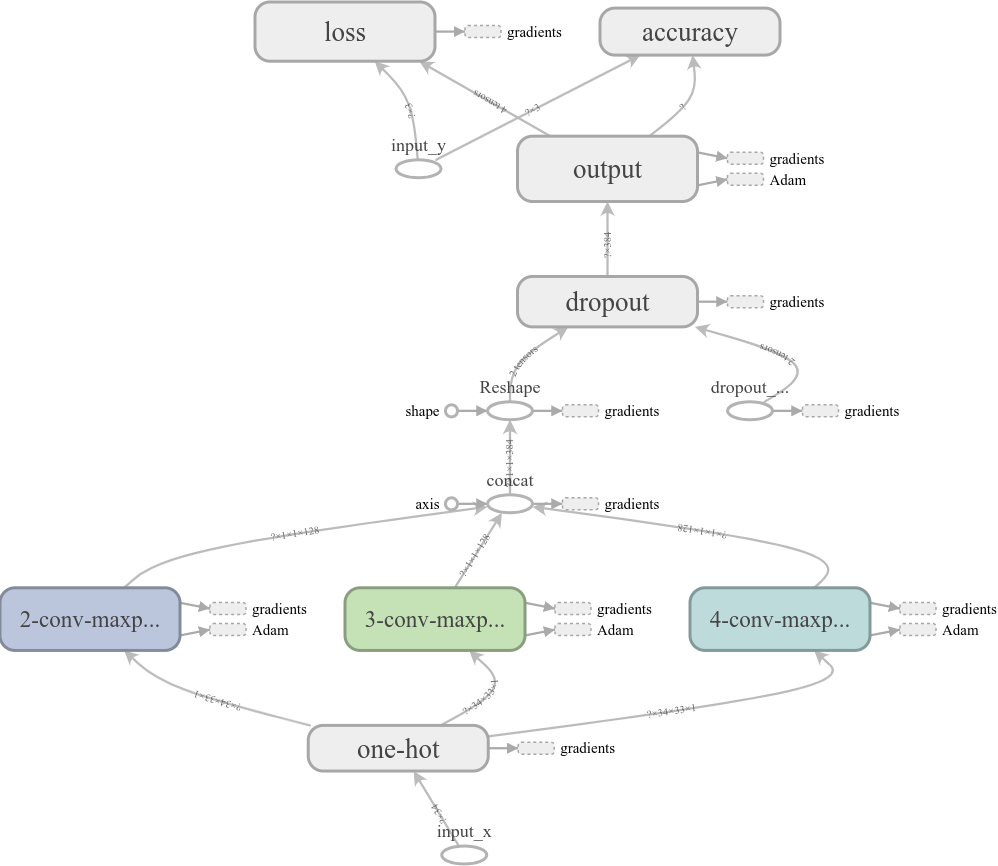
\includegraphics[width=.7\linewidth]{cnn_1}}
	\hfill
	\subbottom[\label{img:cnn-struct2}]{%
		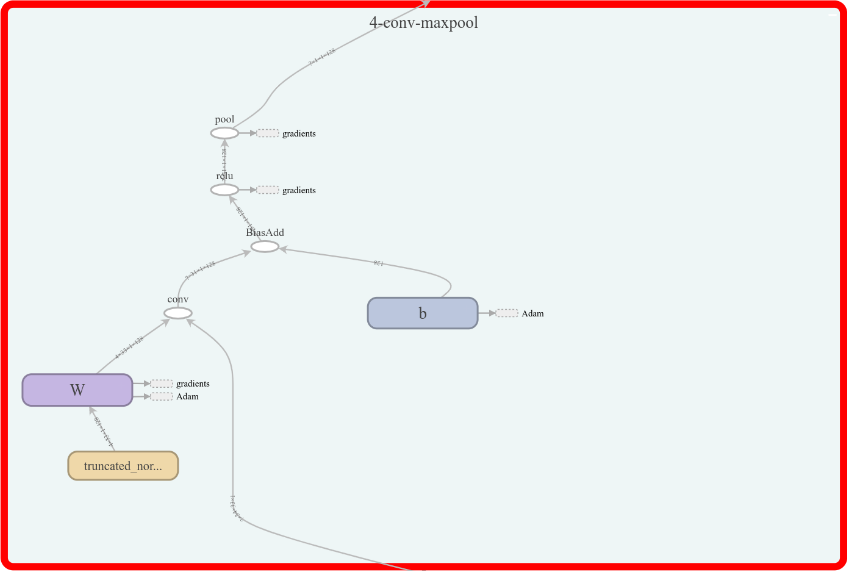
\includegraphics[width=.25\linewidth]{cnn_2}}
	\caption{Структура згорткової нейронної мережі (\subcaptionref{img:cnn-struct1}) та деталізація її згорткового шару (\subcaptionref{img:cnn-struct2})}
	\label{img:cnn-struct}
\end{figure}

Фонеми представлені у вигляді one-hot вектору. Фрази нормалізовані за максимальною довжиною, з використанням вектора з усіма нулями в якості заповнювача.

На відміну від роботи по словам, вкладений шар (embedding layer) відсутній, оскільки потужність множини фонем набагато нижчий ніж потужність множини слів, і такий шар не є необхідним. З іншого боку, деякі фонеми схожі на інші, а деякі ні, тому використання вкладень може бути доцільним для передачі цієї схожості, а не тільки для зниження розмірності. Навчання вкладеного шару потребує великого обʼєму вхідних даних, тому в даній роботі не буде розглянуто.

Використовується комбінований згортковий шар (convolution layer), який складається з декількох паралельних одновимірних шарів з різними варіантами кроку фільтра.

Для агрегації кожного зі згорткових шарів використовується агрегаційний шар (pooling layer) з вибором одного максимального значення (1-max-pooling).

Виходи агрегаційних підшарів різного розміру кроку згортки комбінується в один вектор значень.

У якості повнозвʼязного шару використовується класичний перцептрон, який може мати активаційну функцію у вигляді не спадаючих диференційованих функцій, що діють на множині дійсних чисел. У нашому випадку для функції активації використаємо ReLU:

\[
h(a) = \max(0, a),
\]

\noindent
де $a=WX+b$

Застосування у якості функції активації ReLU дозволяє забезпечити головні переваги, які надають можливість здійснити пришвидшення навчання нейронної мережі через розрідженість та меншу величину ймовірності розмиття градієнту в порівнянні з іншими активаційними функціями. Виникнення розрідженості відбувається при значеннях a < 0. Для більшої кількості нейронів з ReLU-активацією в шарі характерна більша розрідженість отриманого результату.

Для зниження ефекту перенавчання використовується Dropout шар.

Традиційно для задач класифікації в якості функції втрат використовується кросс-ентропія. Інакше кажучи, робимо мінімізацію різниці між виходом нейронної мережі і відповідною фонемою (контекстом). Різницею, якраз і буде величина кросс-ентропії, яка визначається за наступною формулою:

\[
D(\hat{y},y)=-\sum_j y_i \ln \hat{y}_i
\]

Для навчання використовується Adam-алгоритм зворотного розповсюдження помилки із стохастичним градієнтним спуском, який дозволяє регулювати величину швидкості навчання в залежності від параметрів з виконанням більших оновлень для 32-х або 16-ти рідких параметрів і маленьких оновлень для більш частих параметрів \cite{Kingma_2014}. У даному методі використовуються накопичені значення градієнтів, що отримані на попередніх кроках, і накопичені значення квадратів градієнтів. Сам процес накопичення протікає на основі експоненціального розпаду середніх значень (EDAverage). Самі значення, що отримані на останньому кроці мають найбільший внесок для сумарного вихідного значення в порівнянні із значеннями градієнтів, що отримані на перших кроках:

\[
\bar{m_t}=\beta_1m_{t-1}+(1-\beta_1)g_t;
\]

\[
\bar{v_t}=\beta_2v_{t-1}+(1-\beta_2)g^2_t,
\]

\noindent
де $\bar{m_t}$ – середня оцінка першого моменту; $\bar{v_t}$ – середня оцінка другого моменту.

Оскільки у вищеприведених формулах констатація величин $\bar{m_t}$ і $\bar{v_t}$ може бути ініціалізована нулями, то виходить, що вони мають тяжіння до нулів. Таке тяжіння сильно проявляється на початкових кроках і, коли величина коефіцієнтів розпаду приймає мале значення ($\beta_1$ і $\beta_2$). Для вирішення цієї проблеми на значення моментів накладається штраф:

\[
\hat{m}_t=\frac{m_t}{1-\beta_1^t};
\]

\[
\hat{v}_t=\frac{v_t}{1-\beta_2^t}.
\]

Величини отриманих значень використовуються в процесі оновлення нових параметрів на основі формули:

\[
\Theta_{t+1}=\Theta_t-\frac{\eta}{\sqrt{\hat{v}_t}+\varepsilon}\hat{m}_t.
\]

%Розглянемо принцип побудови алгоритму зворотного поширення помилки ЗНМ. У випадку запропонованої ЗНМ їй характерний і достатній в наявності один паралельний одновимірний шар. Нехай $W$ – матриця вагових коефіцієнтів, які характеризують звʼязок виходів і входу паралельних шарів, а $V$ – матриця вагових коефіцієнтів, які зʼєднують вихід паралельного шару і вихідний. Індекси для входу – $i$, індекси елементів паралельного нейронного шару – $j$, а індекси виходів – $k$.
%
%У ЗНМ відбувається навчання на наборах фонем ($X_a$ – один з елементів множини фонем $M$) і реакцій на них ($Y_a$ – один з елементів множини реакцій), $a = 1...p$. При цьому величинами активності нейронів є $y$, а сумарні зважені входи нейронів – $x$ з відповідними індексами.
%
%При алгоритмі зі зворотним поширенням помилки в ЗНМ матимемо наступні кроки:
%
%Крок 1. Вважаємо, що початковим значенням ваг для двох нейронів одного паралельного шару при $t = 0$ притаманні випадкові числа.
%
%Крок 1. Відбувається подача one-hot вектору фонем $X_a$ у ЗНМ, в результаті відбувається формування вихідного вектору ймовірності вибору команди $Y_a$. Тоді функціонування нейронів проходить послідовні етапи від шару до шару на підставі наступних формул:
%
%\begin{itemize}
%	\item у першому паралельному шарі:
%\end{itemize}
%
%\[
%x_j=\sum_i{W_{ij}X_i^a},
%\]
%
%\begin{itemize}
%	\item у вихідному шарі:
%\end{itemize}
%
%\[
%x_k=\sum_i{V_{ik}y_i}; y_k=f(x_k).
%\]
%
%В останній формулі $f(х)$ являє собою неспадну функцію ReLU.
%
%Крок 2. Приймаємо, що для вхідного вектору ймовірності вибору команди значення функціоналу квадратичної помилки ЗНМ має наступний вигляд:
%
%\[
%E=\frac{1}{2}\sum_k{\left(y_k-Y_k^a\right)^2}.
%\]
%
%Проведемо обовʼязкову мінімізацію наведеного функціоналу за допомогою класичного градієнтного методу, для якого характерним є ітераційний процес уточнення аргументу, який виконується відповідно до формули:
%
%\[
%V_{jk}(t+1)=V_{jk}(t)-h\frac{\partial E}{\partial V_{jk}}.
%\]
%
%Бачимо, що в складі функції помилки  класифікації голосових команд відсутні залежності від ваги $V_{jk}$ в явному виді, тому використовуємо формули неявного диференціювання для складної функції:
%
%\[
%\frac{\partial E}{\partial y_k}=\delta_k=\left ( y_k-Y_k^a \right );
%\]
%
%\[
%\frac{\partial E}{\partial x_k}=\frac{\partial E}{\partial y_k}\frac{\partial y_k}{\partial x_k}=\delta_ky_k(1-y_k);
%\]
%
%\[
%\frac{\partial E}{\partial V_{jk}}=\frac{\partial E}{\partial y_k}\frac{\partial y_k}{\partial x_k}\frac{\partial x_k}{\partial V_{jk}}=\delta_ky_k(1-y_k)y_i.
%\]
%
%Крок 3. Виконаємо підстроювання ваг паралельного шару ЗНМ. Для цього будемо використовувати градієнтний метод:
%
%\[
%W_{jk}(t+1)=W_{jk}(t)-h\frac{\partial E}{\partial W_{jk}}
%\]
%
%Аналогічно виконуємо обчислення похідних, але вже з деякими ускладненнями формули, призначеної для помилки :
%
%\[
%\frac{\partial E}{\partial x_k}=\frac{\partial E}{\partial y_k}\frac{\partial y_k}{\partial x_k}=\delta_ky_k(1-y_k);
%\]
%
%\[
%\frac{\partial E}{\partial y_j}=\delta_j=\sum_k{\frac{\partial E}{\partial x_k}\frac{\partial x_k}{\partial y_j}}=\sum_k{\delta_ky_k(1-y_k)V_{jk}};
%\]
%
%\[
%\frac{\partial E}{\partial W_{ij}}
%=\frac{\partial E}{\partial y_j}\frac{\partial y_j}{\partial x_j}\frac{\partial x_j}{\partial W_{ij}}
%=\delta_jy_j(1-y_j)X_i^a=\left [ \sum_k{\delta_ky_k(1-y_k)V_{jk}} \right ] \left [ y_j\left(1-y_j\right)X_i^a \right ].
%\]
%
%Під час обчислення $d_j$ застосовується принцип зворотного поширення помилки, тобто тільки за іншими змінними паралельного шару беруться часткові похідні. Далі, за допомогою отриманих виразів відбувається модифікація ваг паралельного нейронного шару ЗНМ.
%
%Крок 4. Надалі, для всіх навчальних етапів повторюються кроки 1-3, а завершення навчання відбувається в тому випадку, коли досягається заданий рівень помилки або досягнута максимально допустима кількість ітерацій. Пройдені 2 і 3-ій кроки допомагають вирішити завдання з оптимізації отриманого функціоналу помилки класифікації голосових команд із застосуванням градієнтного методу з подальшим навчанням ЗНМ. Отримані параметри характеризуються темпами навчання і вибираються з дуже малими значеннями для забезпечення гарантії збіжності застосованого методу.


Отже метод згорткових нейронних мереж для класифікації фонемної репрезентації голосових команд як частину дуальної системи формалізації голосової інформації в системах диспетчерського контролю за рухом автотранспорту можна сформулювати наступним чином:

\begin{enumerate}
	\item представлення кожної фонеми у вигляді one-hot вектору;
	\item розрахунок одновимірного згорткового шару з фільтрами розмірами 2, 3 та 4 і кроком 1;
	\item розрахунок агрегаційного шару виділенням максимального значення кожного фільтру;
	\item конкатенація результатів обрахунку всіх фільтрів;
	\item розрахунок повнозвʼязного шару з функцією активації ReLU та нормалізацією Dropout;
	\item розрахунок точності та функції втрат.
\end{enumerate}

\subsection{Представлення інтелектуальних рефлекторних систем у термінах згорткових нейронних мереж}

Якщо детально розглянути ядро розрахунків РГСУ (розд. \ref{subsect2_4_2}) то видно що воно дуже нагадує повнозвʼязний шар нейронної мережі. Умовна ймовірність вибору реакції $A_i$, при існуванні впливу $B_j$ ($p(A_i/B_j)$) відповідає вагам шару нейронної мережі ($W = |w_ij|$), а безумовна ймовірність вибору реакції $A_i$ ($p(A_i)$) відповідає зміщенням ($B = |b_i|$). На відміну від класичного перцептрону, в якому функція активації застосовується до результата добутку матриць ($Y=f(WX + B)$), функція активації в РГСУ набагато складніша, до того ж працює з вагами та зміщеннями напряму, як наприклад радиально-базисна функція активації.

В оригінальній роботі\cite{Teslia_2014} параметри $p(A_i/B_j)$ та $p(A_i)$ розраховуються частотно. Фактично в оригінальній роботі не було етапу навчання аналогічного до такого при навчанні нейронних мереж. Такий підхід більше схожий на метод найменших квадратів, де параметри можуть бути напряму вирахувані і не потребують оптимізації.
Але якщо обмежити діапазон можливих значень параметрів інтервалом $[0, 1]$ який відповідає можливим значенням ймовірності, то можна спробувати отримати оптимальні значення цих параметрів шляхом навчання методом зворотного розповсюдження помилки.

Для цього представимо метод інтелектуальних рефлекторних систем для класифікації голосових команд у матричній формі:

\begin{enumerate}
	\item Розрахунок визначеності для інтелектуальної системи відносно всіх вхідних N-грам фонем і можливих голосових команд:
	
	\begin{align}
		D_A&=\pm0.5(P_{A}\oslash(J_{1,p}-P_{A}) + (J_{1,p}-P_{A})\oslash P_{A} -2J_{1,p})^{\circ \frac{1}{2}}; \nonumber \\
		D_{AB}&=\pm0.5(P_{AB}\oslash(J_{p,q}-P_{AB}) + (J_{p,q}-P_{AB})\oslash P_{AB}-2J_{p,q})^{\circ \frac{1}{2}}; \nonumber \\
		I_A&=(D_A^{\circ 2}+J_{1,p})^{\circ \frac{1}{2}};\quad I_{AB}=(D_{AB}^{\circ 2}+J_{p,q})^{\circ \frac{1}{2}}, \nonumber
	\end{align}
	
	де: $p=|A|$ --- потужність множини голосових команд;
	
	{\settowidth{\leftskip}{де:\ }
		
		$q=|B|=\sum_{i=s_{\text{min}}}^{s_{\text{max}}}f^i$ --- потужність множини N-грам фонем,
		
		$f$ --- кількість фонем в акустичній моделі,
		
		$s_{\text{min}}$ та $s_{\text{max}}$ --- мінімальний та максимальний розміри N-грам;
		
		$J_{i,j}$ --- матриця одиниць розміром $i\times j$
		
		$P_{A}$ --- матриця безумовної ймовірності вибору команд з множини $A$ (розмір матриці $1\times p$); 
		
		$D_A$ --- матриця визначеності щодо команд з множини $A$; 
		
		$I_A$ --- матриця інформованості щодо команд з множини $A$; 
		
		$P_{AB}$ --- матриця умовної ймовірності вибору команд з множини $A$ при наявності впливу N-граму фонем з множини $B$ (розмір матриці $p\times q$); 
		
		$D_{AB}$ --- матриця визначеності щодо команд з множини $A$ при наявності впливу N-граму фонем з множини $B$; 
		
		$I_{AB}$ --- матриця інформованості щодо команд з множини $A$ при наявності впливу N-граму фонем з множини $B$
		
		$\circ$, ${}^{\circ}$ та $\oslash$ --- операції матричного поелементного добутку, піднесення до степеня та ділення Адамара.
		
	}
	
	\item Отримання додаткової визначеності, що є у N-грамів фонем відносно голосових команд:
	
	\[
	D_\Delta=D_{AB} \circ (J_{p,1}I_A)-I_{AB} \circ (J_{p,1}D_A),
	\]
	
	де $D_\Delta$ --- матриця додаткової визначеності щодо команд з множини $A$ яку надає наявність N-граму фонем з множини $B$ (розмір матриці $p\times q$).
	
	\item Розрахунок сумарного впливу на голосову команду, реакцію інтелектуальної системи всіх наявних N-грамів фонем:
	
	\[
	D_\Sigma = XD_\Delta;\quad I_\Sigma=(D_\Sigma^{\circ 2}+J_{n,q})^{\circ \frac{1}{2}},
	\]
	
	де: $n$ --- кількість вхідних команд для розпізнання або навчання системи; 
	
	{\settowidth{\leftskip}{де:\ }
		
		$X$ --- вхідна матриця команд для розпізнання або навчання системи представлений у форматі «мішок N-грам фонем», тобто матриці розміром $n \times p$, де $x_{ij}=1$ якщо для відповідної голосової команди $i$ існує N-грам фонем $j$, в інакшому випадку $x_{ij}=0$;
		
		$D_\Sigma$ --- матриця сумарної додаткової визначеності щодо команд  з множини $A$ під впливом всіх N-грамів фонем з множини $B$ (розмір матриці $n\times q$);
		
		$I_\Sigma$ --- матриця сумарної додаткової інформованості щодо команд  з множини $A$ під впливом всіх N-грамів фонем з множини $B$.
		
	}
	
	\item Обчислення нової інформованості та визначеності голосової команди:
	
	\[
	D_Y=D_\Sigma \circ (J_{n,1}I_A) - I_\Sigma \circ (J_{n,1}D_A);\quad I_Y=(D_Y^{\circ 2}+J_{n,q})^{\circ \frac{1}{2}},
	\]
	
	де $D_Y$ --- матриця нової (вихідної) визначеності щодо команд  з множини $A$ під впливом всіх N-грамів фонем з множини $B$ (розмір матриці $n\times q$); 
	
	$I_Y$ --- матриця нової (вихідної) щодо команд з множини $A$ під впливом всіх N-грамів фонем з множини $B$.
	
	\item Обчислення сумісної умовної ймовірності команди $A_i$ (при наявності всіх N-грамів фонем $B_j \in B$):
	
	\[
	Y=P_Y=0.5J_{n,p}+D_Y \oslash 2I_Y,
	\]
	
	де $P_Y$ --- матриця сумісної умовної ймовірності команд з множини $A$ під впливом всіх N-грамів фонем з множини $B$.
\end{enumerate}

Попередня обробка фонем (обʼєднання послідовних наборів фонем різної довжини) відповідає згортковим та агрегаційним шарам згорткової нейронної мережі, але замість підбору найкращих фільтрів, використовується фіксований набір. Він включає в себе всі можливі комбінації фонем відповідно до розміру вікна фільтру. Такий фіксований набір фільтрів одночасно є набагато більшим за необхідний для ефективного розпізнавання і при цьому не достатньо повним, оскільки не включає нелінійні комбінації та пропуски, коли деякі фонеми у вікні фільтра важливіші. Тому навчання оптимальних параметрів фільтру в нейронній мережі може дати кращий результат.

Функція активації РГСУ достатньо складна, і її розрахунок набагато довший ніж ReLU чи інші функції активації  повнозвʼязних шарів. Оскільки в класичному підході РГСУ немає ітеративного навчання, це не є критичною проблемою. Але саме порівняння інтроформаційної функції активації з класичними функціями нелінійності нейронних мереж в рівних умовах, може дати незалежну оцінку її ефективності. 

\section*{Висновки до розділу 3}
\addcontentsline{toc}{section}{Висновки до розділу 3}

1. Запропонована класифікація реакцій для субʼєктів дистрибуції на етапах «склад – дорога – точка доставки» базується на зібраних статистичних даних (зауваженнях та оригінальних коментарях) щодо процесу доставки різних вантажів автомобільним транспортом у провідних логістичних компаніях України.

%1. Під час розгляду методів формалізації голосової інформації в системах диспетчерського контролю за рухом автотранспорту зібрано статистичні дані (зауваження та оригінальні коментарі) щодо процесу доставки різних вантажів автомобільним транспортом у провідних логістичних компаніях України. Після систематизації та обробки даних запропоновано класифікацію реакцій для субʼєктів дистрибуції «склад – дорога – точка доставки».

2. Розроблено модель голосової взаємодії субʼєктів дистрибуції в системах диспетчерського контролю за рухом автотранспорту, яка представлена у вигляді повного графу сценаріїв усіх етапів дистрибуції. 

3. Виділено перелік унікальних контекстів голосової взаємодії, формалізація голосової інформації в яких може відбуватися незалежно, що дозволяє знизити кількість реакцій для розпізнання.

%2. Розроблено дерево сценаріїв усіх етапів дистрибуції «склад – дорога – точка доставки» як модель голосової взаємодії водія в системах диспетчерського контролю за рухом автотранспорту та визначено перелік контекстів та можливих реакцій на них.

4. Створено метод формалізації голосової інформації в системах підтримки диспетчеризації автотранспорту з використанням інтелектуальних рефлекторних систем, що дозволяє автоматизувати голосову взаємодію субʼєктів дистрибуції з уникненням переводу звукової інформації в лексичний текст за рахунок використання двох основних модулів (автоматичного фонетичного стенографа і ядра рефлекторної системи голосового управління).

%3. Для формалізації голосової інформації запропоновано використання методу формалізації голосової інформації в моделі голосової взаємодії водія при диспетчерському контролі за рухом автотранспорту, що складається з двох основних модулів: автоматичного фонетичного стенографа і ядра рефлекторної системи голосового управління, поточна реалізація яких визначає умови їх використання в моделі голосової взаємодії. При використанні такої системи не потрібно створювати ніяких словників, виконувати морфологічний, синтаксичний, семантичний аналіз тексту, а також виділяти слова і команди; вибір реакції відбувається на звуковий потік, з якого система формалізації голосової інформації в моделі голосової взаємодії водія при диспетчерському контролі за рухом автотранспорту, як і людина сама «вміє виділяти» інформативну частину за максимальною визначеністю.

5. Для реалізації ядерного компонента рефлекторної системи голосового управління запропоновано дуальну систему класифікації голосових команд, яка може бути налаштована на предметну область і використовувати метод інтелектуальних рефлекторних систем або метод згорткових нейронних мереж в залежності від того, який показує кращі результати.

6. Метод згорткових нейронних мереж застосовано до фонемного тексту з метою класифікації голосових команд для формалізації голосової інформації в системах диспетчерського контролю за рухом автотранспорту.

%Для формалізації голосової інформації запропоновано використовувати згорткові нейронні мережі. У даному випадку система формалізації голосової інформації в моделі голосової взаємодії водія при диспетчерському контролі за рухом автотранспорту містить фонемний стенограф та згорткову нейронну мережу, яка працює з фонемами. Реалізація ЗНМ виконана на мові Python з використанням TensorFlow. Нейронна мережа містить паралельні одновимірні шари з різними варіантами кроку фільтра з активаційною неспадаючою диференційованою функцією ReLU; фонеми представляються у вигляді one-hot вектору, фрази нормалізовані за максимальною довжиною, з використанням вектора з усіма нулями в якості заповнювача. Для навчання використано Adam-алгоритм зворотного розповсюдження помилки із стохастичним градієнтним спуском, який дозволяє регулювати величину швидкості навчання в залежності від параметрів. Для зниження ефекту перенавчання ЗНМ використано Dropout шар. Також побудовано алгоритм зворотного поширення помилки ЗНМ. 

7. Для формалізації процесів взаємодії метод інтелектуальних рефлекторних систем представлено у термінах нейронних мереж, шо дає можливість отримати оптимальні значення параметрів рефлекторних систем шляхом навчання методом зворотного розповсюдження помилки.

%Крім того, для формалізації голосової інформації запропоновано представляти інтелектуальні рефлекторні системи у термінах згорткових нейронних мереж. При цьому в роботі запропоновано параметри p$(A_i/Bj)$ та $p(A_i)$ розраховувати частотно, при навчанні нейронних мереж не буде аналогічного етапу навчання. Останнє дає можливість отримати оптимальні значення зазначених параметрів шляхом навчання методом зворотного розповсюдження помилки. Тому навчання оптимальних параметрів фільтру в нейронній мережі розкриває можливість отримати кращий результат у порівнянні з існуючими. На жаль, дана розробка лишилась лише теоретичною.